\documentclass[specialist,
substylefile = spbu_report.rtx,
subf,href,colorlinks=true, 12pt]{disser}

\usepackage[T2A]{fontenc}
\usepackage[utf8]{inputenc}
\usepackage[english,russian]{babel}

\usepackage[a4paper,
mag=1000, includefoot,
left=3cm, right=1.5cm, top=2cm, bottom=2cm, headsep=1cm, footskip=1cm]{geometry}

\usepackage{graphicx,subcaption,ragged2e}

\usepackage{caption}

%\setlength{\belowcaptionskip}{-10pt}
%\captionsetup{belowskip=0pt}

\usepackage{booktabs}

\usepackage{amsthm}
\usepackage{amsmath}
\usepackage{amssymb}
\usepackage{hhline}
\usepackage{xcolor}
\usepackage{array}
\usepackage{bbm}
\usepackage{bm}

\theoremstyle{definition}
\newtheorem{definition}{Определение}[chapter]
\newtheorem{algorithm}{Алгоритм}
\newtheorem{remark}{Замечание}[chapter]
\newtheorem{example}{Пример}[chapter]
% \newtheorem{assumption}{Предположение}[section]
\newtheorem{statement}{Утверждение}
\newtheorem{proposition}{Предложение}[chapter]
\newtheorem{corollary}{Следствие}[chapter]

\newcommand{\R}{\mathbb{R}}
\newcommand{\Z}{\mathbb{Z}}
\newcommand{\const}{\mathrm{const}}
\newcommand{\im}{\mathrm{i}}

\usepackage{float}

\usepackage{rotating}

%new calligraphic font for subspaces 
\usepackage{euscript}
\newcommand{\cA}{\EuScript{A}}
\newcommand{\cB}{\EuScript{B}}
\newcommand{\cC}{\EuScript{C}}
\newcommand{\cD}{\EuScript{D}}
\newcommand{\cE}{\EuScript{E}}
\newcommand{\cF}{\EuScript{F}}
\newcommand{\cG}{\EuScript{G}}
\newcommand{\cH}{\EuScript{H}}
\newcommand{\cI}{\EuScript{I}}
\newcommand{\cJ}{\EuScript{J}}
\newcommand{\cK}{\EuScript{K}}
\newcommand{\cL}{\EuScript{L}}
\newcommand{\cM}{\EuScript{M}}
\newcommand{\cN}{\EuScript{N}}
\newcommand{\cO}{\EuScript{O}}
\newcommand{\cP}{\EuScript{P}}
\newcommand{\cQ}{\EuScript{Q}}
\newcommand{\cR}{\EuScript{R}}
\newcommand{\cS}{\EuScript{S}}
\newcommand{\cT}{\EuScript{T}}
\newcommand{\cU}{\EuScript{U}}
\newcommand{\cV}{\EuScript{V}}
\newcommand{\cW}{\EuScript{W}}
\newcommand{\cX}{\EuScript{X}}
\newcommand{\cY}{\EuScript{Y}}
\newcommand{\cZ}{\EuScript{Z}}

%font for text indices like transposition X^\mathrm{T}
\newcommand{\rmA}{\mathrm{A}}
\newcommand{\rmB}{\mathrm{B}}
\newcommand{\rmC}{\mathrm{C}}
\newcommand{\rmD}{\mathrm{D}}
\newcommand{\rmE}{\mathrm{E}}
\newcommand{\rmF}{\mathrm{F}}
\newcommand{\rmG}{\mathrm{G}}
\newcommand{\rmH}{\mathrm{H}}
\newcommand{\rmI}{\mathrm{I}}
\newcommand{\rmJ}{\mathrm{J}}
\newcommand{\rmK}{\mathrm{K}}
\newcommand{\rmL}{\mathrm{L}}
\newcommand{\rmM}{\mathrm{M}}
\newcommand{\rmN}{\mathrm{N}}
\newcommand{\rmO}{\mathrm{O}}
\newcommand{\rmP}{\mathrm{P}}
\newcommand{\rmQ}{\mathrm{Q}}
\newcommand{\rmR}{\mathrm{R}}
\newcommand{\rmS}{\mathrm{S}}
\newcommand{\rmT}{\mathrm{T}}
\newcommand{\rmU}{\mathrm{U}}
\newcommand{\rmV}{\mathrm{V}}
\newcommand{\rmW}{\mathrm{W}}
\newcommand{\rmX}{\mathrm{X}}
\newcommand{\rmY}{\mathrm{Y}}
\newcommand{\rmZ}{\mathrm{Z}}

%tt font for time series
\newcommand{\tA}{\mathsf{A}}
\newcommand{\tB}{\mathsf{B}}
\newcommand{\tC}{\mathsf{C}}
\newcommand{\tD}{\mathsf{D}}
\newcommand{\tE}{\mathsf{E}}
\newcommand{\tF}{\mathsf{F}}
\newcommand{\tG}{\mathsf{G}}
\newcommand{\tH}{\mathsf{H}}
\newcommand{\tI}{\mathsf{I}}
\newcommand{\tJ}{\mathsf{J}}
\newcommand{\tK}{\mathsf{K}}
\newcommand{\tL}{\mathsf{L}}
\newcommand{\tM}{\mathsf{M}}
\newcommand{\tN}{\mathsf{N}}
\newcommand{\tO}{\mathsf{O}}
\newcommand{\tP}{\mathsf{P}}
\newcommand{\tQ}{\mathsf{Q}}
\newcommand{\tR}{\mathsf{R}}
\newcommand{\tS}{\mathsf{S}}
\newcommand{\tT}{\mathsf{T}}
\newcommand{\tU}{\mathsf{U}}
\newcommand{\tV}{\mathsf{V}}
\newcommand{\tW}{\mathsf{W}}
\newcommand{\tX}{\mathsf{X}}
\newcommand{\tY}{\mathsf{Y}}
\newcommand{\tZ}{\mathsf{Z}}

%bf font for matrices
\newcommand{\bfA}{\mathbf{A}}
\newcommand{\bfB}{\mathbf{B}}
\newcommand{\bfC}{\mathbf{C}}
\newcommand{\bfD}{\mathbf{D}}
\newcommand{\bfE}{\mathbf{E}}
\newcommand{\bfF}{\mathbf{F}}
\newcommand{\bfG}{\mathbf{G}}
\newcommand{\bfH}{\mathbf{H}}
\newcommand{\bfI}{\mathbf{I}}
\newcommand{\bfJ}{\mathbf{J}}
\newcommand{\bfK}{\mathbf{K}}
\newcommand{\bfL}{\mathbf{L}}
\newcommand{\bfM}{\mathbf{M}}
\newcommand{\bfN}{\mathbf{N}}
\newcommand{\bfO}{\mathbf{O}}
\newcommand{\bfP}{\mathbf{P}}
\newcommand{\bfQ}{\mathbf{Q}}
\newcommand{\bfR}{\mathbf{R}}
\newcommand{\bfS}{\mathbf{S}}
\newcommand{\bfT}{\mathbf{T}}
\newcommand{\bfU}{\mathbf{U}}
\newcommand{\bfV}{\mathbf{V}}
\newcommand{\bfW}{\mathbf{W}}
\newcommand{\bfX}{\mathbf{X}}
\newcommand{\bfY}{\mathbf{Y}}
\newcommand{\bfZ}{\mathbf{Z}}

%bb font for standard spaces and expectation
\newcommand{\bbA}{\mathbb{A}}
\newcommand{\bbB}{\mathbb{B}}
\newcommand{\bbC}{\mathbb{C}}
\newcommand{\bbD}{\mathbb{D}}
\newcommand{\bbE}{\mathbb{E}}
\newcommand{\bbF}{\mathbb{F}}
\newcommand{\bbG}{\mathbb{G}}
\newcommand{\bbH}{\mathbb{H}}
\newcommand{\bbI}{\mathbb{I}}
\newcommand{\bbJ}{\mathbb{J}}
\newcommand{\bbK}{\mathbb{K}}
\newcommand{\bbL}{\mathbb{L}}
\newcommand{\bbM}{\mathbb{M}}
\newcommand{\bbN}{\mathbb{N}}
\newcommand{\bbO}{\mathbb{O}}
\newcommand{\bbP}{\mathbb{P}}
\newcommand{\bbQ}{\mathbb{Q}}
\newcommand{\bbR}{\mathbb{R}}
\newcommand{\bbS}{\mathbb{S}}
\newcommand{\bbT}{\mathbb{T}}
\newcommand{\bbU}{\mathbb{U}}
\newcommand{\bbV}{\mathbb{V}}
\newcommand{\bbW}{\mathbb{W}}
\newcommand{\bbX}{\mathbb{X}}
\newcommand{\bbY}{\mathbb{Y}}
\newcommand{\bbZ}{\mathbb{Z}}

%got font for any case
\newcommand{\gA}{\mathfrak{A}}
\newcommand{\gB}{\mathfrak{B}}
\newcommand{\gC}{\mathfrak{C}}
\newcommand{\gD}{\mathfrak{D}}
\newcommand{\gE}{\mathfrak{E}}
\newcommand{\gF}{\mathfrak{F}}
\newcommand{\gG}{\mathfrak{G}}
\newcommand{\gH}{\mathfrak{H}}
\newcommand{\gI}{\mathfrak{I}}
\newcommand{\gJ}{\mathfrak{J}}
\newcommand{\gK}{\mathfrak{K}}
\newcommand{\gL}{\mathfrak{L}}
\newcommand{\gM}{\mathfrak{M}}
\newcommand{\gN}{\mathfrak{N}}
\newcommand{\gO}{\mathfrak{O}}
\newcommand{\gP}{\mathfrak{P}}
\newcommand{\gQ}{\mathfrak{Q}}
\newcommand{\gR}{\mathfrak{R}}
\newcommand{\gS}{\mathfrak{S}}
\newcommand{\gT}{\mathfrak{T}}
\newcommand{\gU}{\mathfrak{U}}
\newcommand{\gV}{\mathfrak{V}}
\newcommand{\gW}{\mathfrak{W}}
\newcommand{\gX}{\mathfrak{X}}
\newcommand{\gY}{\mathfrak{Y}}
\newcommand{\gZ}{\mathfrak{Z}}

%old calligraphic font
\newcommand{\calA}{\mathcal{A}}
\newcommand{\calB}{\mathcal{B}}
\newcommand{\calC}{\mathcal{C}}
\newcommand{\calD}{\mathcal{D}}
\newcommand{\calE}{\mathcal{E}}
\newcommand{\calF}{\mathcal{F}}
\newcommand{\calG}{\mathcal{G}}
\newcommand{\calH}{\mathcal{H}}
\newcommand{\calI}{\mathcal{I}}
\newcommand{\calJ}{\mathcal{J}}
\newcommand{\calK}{\mathcal{K}}
\newcommand{\calL}{\mathcal{L}}
\newcommand{\calM}{\mathcal{M}}
\newcommand{\calN}{\mathcal{N}}
\newcommand{\calO}{\mathcal{O}}
\newcommand{\calP}{\mathcal{P}}
\newcommand{\calQ}{\mathcal{Q}}
\newcommand{\calR}{\mathcal{R}}
\newcommand{\calS}{\mathcal{S}}
\newcommand{\calT}{\mathcal{T}}
\newcommand{\calU}{\mathcal{U}}
\newcommand{\calV}{\mathcal{V}}
\newcommand{\calW}{\mathcal{W}}
\newcommand{\calX}{\mathcal{X}}
\newcommand{\calY}{\mathcal{Y}}
\newcommand{\calZ}{\mathcal{Z}}


\setcounter{tocdepth}{2}

\begin{document}

%
% Титульный лист на русском языке
%
% Название организации
\institution{%
	Санкт-Петербургский государственный университет\\
	Прикладная математика и информатика
}

\title{Отчет по учебной практике 1 (проектно-технологическая) (семестр 1)}

% Тема
\topic{Метод Monte Carlo SSA для процессов с длинной памятью}

% Автор
\author{Потешкин Егор Павлович}
\group{группа 24.M22-мм}

% Научный руководитель
\sa       {Голяндина Нина Эдуардовна \\%
	Кафедра Статистического Моделирования}
\sastatus {д.\,ф.-м.\,н., доцент}

% Город и год
\city{Санкт-Петербург}
\date{\number\year}

\maketitle

\tableofcontents

\intro
Метод Singular Spectrum Analysis (SSA)~\cite{Broomhead1986,Golyandina2001} является мощным инструментом для анализа временных рядов. Он позволяет разложить ряд на интерпретируемые компоненты, такие как тренд, периодические колебания и шум, что значительно упрощает процесс анализа. Метод Monte Carlo SSA~\cite{Allen1996}, в свою очередь, решает задачу обнаружения сигнала в шуме, проверяя соответвующую гипотезу.

Для наиболее распространенного варианта метода Monte Carlo SSA необходимо, чтобы спектральная плотность шума была строго монотонной. Такое ограничение связано с методом SSA и понятием строгой разлелимости компонент, без которой оценить доминирующую частоту значимой компоненты не представляется возможным.

В большинстве работ, посвященных методу Monte Carlo SSA, в качестве шума используется модель красного шума~--- процесса авторегрессии первого порядка с положительным коэффициентом. Такая модель шума обладает строго монотонной спектральной плотностью, однако она плохо описывает временные ряды, обладающие длинной памятью, то есть ряды, автоковариционная функция которых убывает медленней, чем экспоненциальное затухание. Процессы с длинной памятью довольно распространены в реальном мире, например, в работе~\cite{Hipel1994} обнаружена длинная память в таких среднегодовых гидрологических временных рядах, как количество осадков, температура и данных о речном стоке. В работе~\cite{Haslett1989} на наличие длинной памяти исследовалась скорость ветра в Ирландии, в работе~\cite{Mariani2020} исследовался эффект длинной памяти у сейсмических данных. Помимо геофизики, длинная память встречается также в финансах~\cite{Barkoulas1997,Guglielmo2019}.

Помимо проблемы выбора модели шума, существует проблема оценки параметров рассматриваемой модели. В реальных задачах редко встречается ситуация, когда параметры известны, поэтому параметры необходимо наилучшим образом оценить на основе исходного временного ряда. Неправильно оцененные параметры модели могут значительно повлиять на результат Monte Carlo SSA.

В данной работе была расширена применимость метода Monte Carlo SSA на временные ряды с длинной памятью. Также, поскольку истинные параметры модели для конкретного временного ряда неизвестны почти всегда, было произведено численное сравнение различных методов оценки параметров. 

% Опишем структуру работы.

% В главе~\ref{chpt:processes} приведено понятие процессов с длинной памятью, также описаны методы оценки параметров модели $\mathrm{ARFIMA}(p, d, q)$, одного из распространенных процессов с длинной памятью, и численное сравнение этих методов. В главе~\ref{chpt:mcssa} представлены методы SSA и Monte Carlo SSA, и проведено численное сравнение метода Monte Carlo SSA с моделями красного шума и $\mathrm{ARFIMA}(0, d, 0)$, обладающими одинаковой дисперсией. Помимо этого, в этой главе продемонстрированы примеры применения метода на реальных данных, обладающих длинной памятью.
\chapter{Теория случайных процессов}\label{chpt:processes}
\section{Вспомогательные определения}
Для начала введем некоторые обозначения, которые будем использовать в дальнейшем.
\begin{definition}\label{def:stationary}
	Случайный процесс $\{Y_t:t\in\Z\}$ называют стационарным (в широком смысле), если
	\begin{enumerate}
		\item $\mathsf{E}Y_t\equiv\const$ (среднее постоянно по времени);
		\item $\mathsf{cov}(Y_t,Y_{t+h})=\gamma(h)$ (ковариация зависит только от лага $h$).
	\end{enumerate}
\end{definition}
\begin{remark}
	Поскольку $\gamma(0)=\mathsf{cov}(Y_t,Y_t)=\mathsf{D}Y_t$, то дисперсия также не меняется со временем.
\end{remark}
\begin{remark}
	Далее под стационарностью будет подразумеваться именно стационарность в широком смысле.
\end{remark}
\begin{definition}
	Случайный процесс $\{\varepsilon_t\}$ называют белым шумом $\mathrm{WN}(0, \sigma^2)$, если он стационарный, $\mathsf{E}\varepsilon_t=0$, $\gamma(h)=0$ $\forall h\ne 0$ и $\mathsf{D}\varepsilon_t=\sigma^2$.
\end{definition}

\begin{definition}
	Моделью $\mathrm{ARMA}(p, q)$, где $p$, $q\in \mathbb{N}\cup\{0\}$ называют случайный процесс $\{X_t\}$, удовлетворяющий соотношению
	\[
		X_t=\varepsilon_t + \sum_{i=1}^p \phi_i X_{t-i} + \sum_{i=1}^q\theta_i\varepsilon_{t-i},
	\]
	где $\{\varepsilon_t\}\sim\mathrm{WN}(0, \sigma^2)$.
\end{definition}
\begin{remark}
	Модель $\mathrm{ARMA}(p, q)$ является стационарным и обратимым процессом, если корни характеристических полиномов
	\[
		\Phi(L)=1-\sum_{i=1}^p \phi_i L^i,\quad \Theta(L)=1+\sum_{i=1}^q \theta_i L^i
	\]
	 лежат вне единичной окружности $\{z:|z|=1\}$~\cite[Section 3.4.1]{BoxJenkins2016}.
\end{remark}

\begin{definition}
	Процесс $\{X_t\}$ называют красным шумом с параметрами $\phi$ и $\sigma^2$, если $\{X_t\}$~--- стационарная модель $\mathrm{ARMA}(p, q)$ с $p=1$, $q=0$ и $\phi=\phi_1\in(0, 1)$.
\end{definition}

\begin{definition}
	Спектральной плотностью стационарного процесса называется такая функция $f(\omega)$, что
	\[
		\gamma(h)=2\int_{0}^{1/2} e^{2\pi h\omega\im}f(\omega)d\omega.
	\]
\end{definition}
\begin{definition}
	Пусть $\{Y_t\}$~--- cтационарный процесс. Функцию
	\[
		I(\omega)=\frac1n\left|\sum_{j=1}^{n} Y_je^{-2\pi \omega j\mathrm{i}}\right|^2
	\]
	называют периодограммой выборки размера $n$ процесса $\{Y_t\}$.
\end{definition}
\begin{remark}
	Для любой фиксированной частоты $\omega_0$
	\begin{align*}
		\mathsf{E}\left(I(\omega_0)\right)\to f(\omega_0),\quad &n\to \infty;\\
		\mathsf{D}\left(I(\omega_0)\right)\to f^2(\omega_0)\ne0,\quad &n\to\infty.
	\end{align*}
	Таким образом периодограмма является асимптотически несмещенной, но несостоятельной, оценкой спектральной плотности~\cite[Раздел 4.5]{Hassler2018}. 
\end{remark}

\section{Процессы с длинной памятью}
\begin{definition}\label{def:longmemory}
	Говорят, что стационарный процесс $\{Y_t\}$ обладает длинной памятью, если
	\[
		\sum_{h=0}^H|\gamma(h)|\to\infty,
	\]
	при $H\to\infty$. Иначе говорят, что $\{Y_t\}$ обладает короткой памятью:
	\[
		\sum_{h=0}^\infty|\gamma(h)|<\infty.
	\]
\end{definition}
Существуют и альтернативные определения процессов с длинной памятью, которые можно найти в~\cite[Раздел 3.1]{Palma2006}. Там же показано, что они согласованы с определением~\ref{def:longmemory}.
% \begin{enumerate}
%     \item Процесс с длинной памятью можно определить как процесс с гиперболическим затуханием автоковариационной функции:
%     \[
%     \gamma(h)\sim h^{2d-1}\ell_1(h),
%     \]
%     при $h\to \infty$, где $d$ так называемый параметр длинной памяти и $\ell_1(\cdot)$~--- медленно меняющаяся на бесконечности функция.
%     \item Также его можно определить поведением спектральной плотности в окрестности нуля:
%     \[
%     f(\lambda)\sim|\lambda|^{-2d}\ell_2(1/|\lambda|),
%     \]
%     при $\lambda\to0$, где $\ell_2(\cdot)$~--- медленно меняющаяся на бесконечности функция.
% \end{enumerate}
\begin{example}
	Процессом с короткой памятью является, например, стационарная модель $\mathrm{ARMA}(p, q)$, поскольку $|\gamma(h)|\leqslant CR^h$, где $C>0$ и $0<R<1$~\cite[Section 10.4]{BoxJenkins2016}.
\end{example}
% Примером стационарного процесса с длинной памятью является дробно интегрированный процесс.
Введем понятие дробного интегрирования $(1-L)^d$, где $L$~--- оператор сдвига. Например, для $d=1$ имеем $(1-L)Y_t=Y_t-Y_{t-1}$, для $d=2$~--- $(1-L)^2Y_t=Y_t-2Y_{t-1}+Y_{t-2}$, и так далее. Обобщим этот оператор для нецелых $d$ с помощью разложения в ряд Тейлора функции $(1-x)^d$ в нуле:
\[
	\begin{aligned}
		(1-x)^d & =1-dx-\frac{d(1-d)}{2}x^2-\frac{d(1-d)(2-d)}{3!}x^3-\ldots             \\
		        & =\sum_{j=0}^\infty \pi_j(d)x^j=\sum_{j=0}^\infty\binom{d}{j}(-1)^jx^j,
	\end{aligned}
\]
где $\binom{d}{j}$~--- обобщенный биномиальный коэффициент. Коэффиенты $\pi_j(d)$ удовлетворяют соотношению
\begin{equation}\label{eq:pi_j}
	\pi_j(d)=(-1)^j\binom{d}{j}=\frac{j-1-d}{j}\pi_{j-1}(d)=\frac{\Gamma(j-d)}{\Gamma(j+1)\Gamma(-d)},
\end{equation}
где $\Gamma(x)$~--- гамма функция. Заметим, что второе равенство в формуле~\eqref{eq:pi_j} верно для любых $d$, третье же верно только для $d\not\in\bbN\cup\{0\}$, поскольку гамма функция не определена для неположительных целых чисел.
% \begin{assumption}\label{as1}
% 	Пусть $\{X_t\}$ представляет собой $\mathrm{MA}(\infty)$ процесс,
% 	\[
% 		X_t=\sum_{j=0}^\infty c_j\varepsilon_{t-j},\quad \{\varepsilon_t\}\sim \mathrm{WN}(0, \sigma^2),
% 	\]
% 	который абсолютно суммируемый, $\sum_{j=0}^\infty |c_j|<\infty$, и $\sum_{j=0}^\infty c_j\ne0$.
% \end{assumption}
% \begin{remark}
%     Данное условие равносильно тому, что $0<f_X(0)<\infty$.
% \end{remark}
\begin{definition}\label{def:arfima}
	Пусть процесс $\{Y_t\}$ определен соотношением
	\[
		\begin{aligned}
			Y_t=(1-L)^{-d}X_t=\sum_{k=0}^\infty \pi_k(-d)X_{t-k}
		\end{aligned},\quad d<1/2,
	\]
	где $\pi_k(-d)$ из формулы~\eqref{eq:pi_j}, $\{X_t\}$~--- стационарная и обратимая модель $\mathrm{ARMA}(p, d)$. Процесс $\{Y_t\}$ называют дробно интегрированной моделью $\mathrm{ARMA}$ или $\mathrm{ARFIMA}(p, d, q)$.
\end{definition}
% \begin{remark}
% 	При $p=q=0$ процесс $\{X_t\}$ из определения~\ref{def:arfima} является белым шумом. В таком случае процесс $\{Y_t\}$ называют дробно интегрированным шумом или $\mathrm{FIN}(d)$.
% \end{remark}

\begin{proposition}\label{prop1}
	Процесс $\{Y_t\}$ из определения~\ref{def:arfima} является стационарным процессом с нулевым средним. Его спектральная плотность определяется выражением
	\begin{equation}\label{eq:spec_long}
		\begin{aligned}
			f_Y(\omega) & =4^{-d}\sin^{-2d}\left(\pi\omega\right)f_X(\omega)                                                                                              \\
			            & =4^{-d}\sin^{-2d}\left(\pi\omega\right)\sigma^2\frac{\left|\Theta(e^{-2\pi \omega\im})\right|^2}{\left|\Phi(e^{-2\pi\omega\im})\right|^2},\quad\omega>0 \\
			            & \sim\omega^{-2d}\sigma^2\frac{|\Theta(1)|^2}{|\Phi(1)|^2},\quad \omega\to0,
		\end{aligned}
	\end{equation}
	где $\Phi(L)$, $\Theta(L)$ --- характеристические полиномы процесса $\{X_t\}$.
\end{proposition}
\begin{proof}
	См.~\cite[Proposition 6.1]{Hassler2018}.
\end{proof}
\begin{remark}
	Из формулы~\eqref{eq:spec_long} видно, что монотонность спектральной плотности процесса $\{Y_t\}$ зависит от поведения спектральной плотности процесса $\{X_t\}$.
\end{remark}
\begin{corollary}\label{corollary1}
	В условиях предложения~\ref{prop1} при $0<d<1/2$
	\[
		\gamma(h)\sim C_{\gamma,d}h^{2d-1},\quad h\to\infty,
	\]
	где
	\[
		C_{\gamma,d}=\sigma^2 \frac{|\theta(1)|^2}{|\phi(1)|^2} \frac{\Gamma(1-2d)}{\Gamma(d)\Gamma(1-d)}.
	\]
\end{corollary}
\begin{proof}
	См.~\cite[Corollary 6.1]{Hassler2018}.
\end{proof}
\begin{remark}
	Из следствия~\ref{corollary1} сразу следует, что $\mathrm{ARFIMA}(p, d, q)$ с $d\in(0, 1/2)$ обладает длинной памятью.
\end{remark}
% \begin{example}
% 	Если $\{X_t\}$ является белым шумом $\mathrm{WN}(0, \sigma^2)$, то $\{Y_t\}$ называют дробно интегрированным шумом ($\mathrm{FIN}$). Его спектральная плотность имеет вид
% 	\[
% 		f_Y(\omega)=\sigma^2 4^{-d}\sin^{-2d}\left(\pi\omega\right).
% 	\]
% 	Отсюда следует, что дробно интегрированный шум всегда обладает монотонной спектральной плотностью.
% \end{example}
% \begin{example}
% 	Стационарный и обратимый $\mathrm{ARMA}$ процесс удовлетворяют предположениям о $\{X_t\}$ в определении~\ref{def:FI}~\cite[Proposition 3.5]{Hassler2018}. Процесс $\{Y_t\}$ в таком случае называют дробно интегрированным $\mathrm{ARMA}$ процессом или коротко $\mathrm{ARFIMA}(p, d, q)$. Его спектральная плотность имеет вид
% 	\[
% 		f_Y(\omega)=\sigma^2 4^{-d}\sin^{-2d}\left(\pi\omega\right)\frac{\left|\theta(e^{-2\pi \omega\im})\right|^2}{\left|\phi(e^{-2\pi\omega\im})\right|^2},
% 	\]
% 	где $\phi$ и $\theta$~--- характеристические полиномы $\mathrm{AR}$ и $\mathrm{MA}$ частей $\mathrm{ARMA}$ соответственно.
% \end{example}

% \subsection{Возникновение процессов с длинной памятью}
% Нас интересуют процессы с монотонной спектральной плотностью, поскольку они довольно распространены в реальном мире. Такими процессами являются процессы со степенной спектральной плотностью $f(\omega)\sim \omega^{-\alpha}$, имеющие большое применение в различных областях, например, в физике, биологии, астрофизике, геофизике и экономике.

% Процессы с длинной памятью, являющиеся частным случаем процессов со степенной спектральной плотностью, довольно распространены. Например, в работе~\cite{Hipel1994} обнаружена длинная память в таких среднегодовых гидрологических временных рядах, как количество осадков, температура и данных о речном стоке. В работе~\cite{Haslett1989} на наличие длинной памяти исследовалась скорость ветра в Ирландии, в работе~\cite{Mariani2020} исследовался эффект длинной памяти у сейсмических данных. Помимо геофизики, длинная память встречается также в финансах~\cite{Barkoulas1997,Guglielmo2019}.

\section{Оценка параметров}
Пусть $Y_t=(1-L)^{-d}X_t$, $d<1/2$. Будем считать, что $\{X_t\}$ представляет собой модель $\mathrm{ARMA}(p, q)$ с нормально распределенным белым шумом $\{\varepsilon_t\}$. Тогда представим его спектральную плотность в параметрическом виде: $f_X(\omega)=f_X(\omega; \bm\psi, \sigma)$, где
\[
	\bm\psi=(\phi_1,\ldots,\phi_p,\theta_1,\ldots,\theta_q)^\rmT.
\]
Поставим задачу оценить параметры $\bm\varphi^\rmT=\left(d, \bm\psi^\rmT\right)$ и $\sigma^2$.

\subsection{Maximum likelihood estimation (MLE)}
Поскольку $\{\varepsilon_t\}$~--- гауссовский белый шум, вектор
\[
	\bm Y=(Y_1,\ldots,Y_n)^\rmT\sim \mathcal{N}_n(\bm0, \bm\Sigma_n),
\]
где $\bm\Sigma_n=(\gamma(|i-j|))_{i,j=1}^n$~--- ковариационная матрица $\bm Y$. Совместная плотность распределения $\bm Y$ равна
\[
	(2\pi)^{-n/2}\left|\bm\Sigma_n\right|^{-1/2}\exp\left\{-\frac12Y^\rmT\bm\Sigma_n^{-1}Y\right\}.
\]
Рассмотрим логарифм функции правдоподобия. Отбрасывая аддитивные константы, получаем
\[
	\ell(\bm\varphi, \sigma^2)=-\frac12\ln\left|\bm\Sigma_n\right|-\frac12 Y^\rmT \bm\Sigma_n^{-1} Y.
\]
Положим $\bm\Gamma_n=\bm\Sigma_n / \sigma^2$ и, максимизируя $\ell$ по $\sigma^2$, получаем
\begin{equation}\label{eq:mle_objective}
	\ell_c(\bm\varphi)=-\frac{n}{2}\ln\left(S(\bm\varphi) / n\right) - \frac{1}{2}\ln g_n(\bm\varphi),
\end{equation}
где $S(\bm\varphi)=\bm Y^\rmT \bm\Gamma_n\bm Y$, $g_n(\bm\varphi)=\left|\bm\Gamma_n\right|$.
Тогда
\[
	\widehat{\bm\varphi}_\mathrm{ML}=\operatorname*{argmax}\limits_{\bm\varphi}\ell_c(\bm\varphi),\quad \widehat\sigma^2_\mathrm{ML} = S(\widehat{\bm\varphi}_\mathrm{ML}).
\]

\begin{remark}
	В случае ненулевого матожидания $\mathsf{E}Y_t=\mu$, для получения $\widehat{\bm\varphi}_\mathrm{ML}$ и $\widehat\sigma^2_\mathrm{ML}$ вместо $\bm Y$ рассматривается $\bm Z=\bm Y-\mu$.
\end{remark}
\begin{remark}
	Для вычисления $\ell_c$ можно использовать алгоритм Левинсона-Дурбина, имеющий временную трудоемкость $O(n^2)$~\cite{McLeod2007}.
\end{remark}
\subsection{Whittle estimation}
Метод максимального правдоподобия применим, когда известно матожидание $\mu$. При неизвестном $\mu$ обычно используют его оценку $\overline{\bm Y}$, однако, помимо этого, существует проблема вычислительной сложности метода при больших $n$.

Обе эти проблемы можно решить, используя оценку Уиттла (Whittle): вместо логарифма функции правдоподобия рассматривается ее оценка (с точностью до константы)~\cite{Whittle1953}. Пусть $f(\omega; \bm\varphi, \sigma^2)$~--- спектральная плотность $\{Y_t\}$, $I(\omega)$~--- периодограмма $\bm Y$, тогда
\[
	\ell_W(\bm\varphi, \sigma^2)=-\frac1m\sum_{j=1}^m\left(\ln f(\omega_j; \bm\varphi, \sigma^2) + \frac{I(\omega_j)}{f(\omega_j; \bm\varphi, \sigma^2)}\right),
\]
где $m=\lfloor(n-1)/2\rfloor$, $\omega_j = j / n$, $j=1,2,\ldots,m$. Заметим, что $f(\omega; \bm\varphi, \sigma^2)=\sigma^2 g(\omega; \bm\varphi)$. Тогда, максимизируя $\ell_W$ по $\sigma^2$, получаем
\[
	\widehat{\bm\varphi}_W = \operatorname*{argmax}_{\bm\varphi}Q(\bm\varphi),\quad \widehat\sigma_W^2=\frac1m \sum_{j=1}^m\frac{I(\omega_j)}{g(\omega_j; \widehat{\bm\varphi}_W)},
\]
где
\[
	Q(\bm\varphi)=-\ln\frac1m \sum_{j=1}^m\frac{I(\omega_j)}{g(\omega_j; \bm\varphi)} - \frac1m \sum_{j=1}^m\ln g(\omega_j; \bm\varphi).
\]
\begin{remark}
	Такой метод оценки параметров можно использовать при неизвестном среднем, поскольку при ее вычислении не используется значение периодограммы в нуле.
\end{remark}
\begin{remark}
	Периодограмму временного ряда можно вычислить за $O(n\log n)$ с помощью быстрого преобразования Фурье, что делает этот метод значительно быстрее MLE для больших $n$.
\end{remark}
\subsection{Численное сравнение методов оценки параметров}\label{sect:est_param}
Сравним качество оценкок параметров следующих моделей:
\begin{enumerate}
	\item $d=q=0$, $p=1$~--- модель $\mathrm{AR}(1)$;
	\item $p=q=0$~--- модель $\mathrm{ARFIMA(0, d, 0)}$.
	\item $p=1$, $q=0$~--- модель $\mathrm{ARFIMA}(1, d, 0)$.
\end{enumerate}
Для оценки параметров этих моделей на языке $\mathsf{R}$~\cite{R} были реализованы функции \textsf{arfima\_mle} и \textsf{arfima\_whittle}, которые соответствуют методам MLE и Whittle соответственно. Для реализации MLE были использованы функции \textsf{tacvfARFIMA} из пакета \textsf{arfima}~\cite{Veenstra2012} и \textsf{DLLoglikelihood} из пакета \textsf{ltsa}~\cite{McLeod2007}, вычисляющие автоковариационную функцию модели ARFIMA и функцию $\ell_c$~\eqref{eq:mle_objective} соответственно. 

Помимо функций \textsf{arfima\_mle} и \textsf{arfima\_whittle}, будем использовать:
\begin{enumerate}
	\item Функцию \textsf{arima} из пакета \textsf{stats}, соответствующую MLE модели ARMA;
	\item Функцию \textsf{fracdiff} из пакета \textsf{fracdiff}~\cite{Maechler1999}, соответствующую апроксимации MLE модели ARFIMA, описанной в работе~\cite{Haslett1989} (обозначим ее за H\&R).
\end{enumerate}
\begin{remark}
	Помимо вышеперечисленных функций, в пакете \textsf{arfima} есть функция \textsf{arfima}, которая вычисляет MLE модели ARFIMA. Но данная реализация MLE в некоторых случаях дает оценки хуже, чем \textsf{arfima\_mle}. Сравнение оценок обоих реализаций можно найти в разделе~\ref{sect:mle_comparison}.
\end{remark}
Поскольку для реальных временных рядов матожидание $\mu$ неизвестно, будем рассматривать MLE с известным средним и с его оценкой~--- выборочным средним (будем обозначать их $\mathrm{MLE}(\mu)$ и $\mathrm{MLE}(\bar x)$ соответственно). Не умаляя общности, пусть $\mu=0$.

\begin{figure}[h]
	\centering
	\begin{subfigure}{\textwidth}
		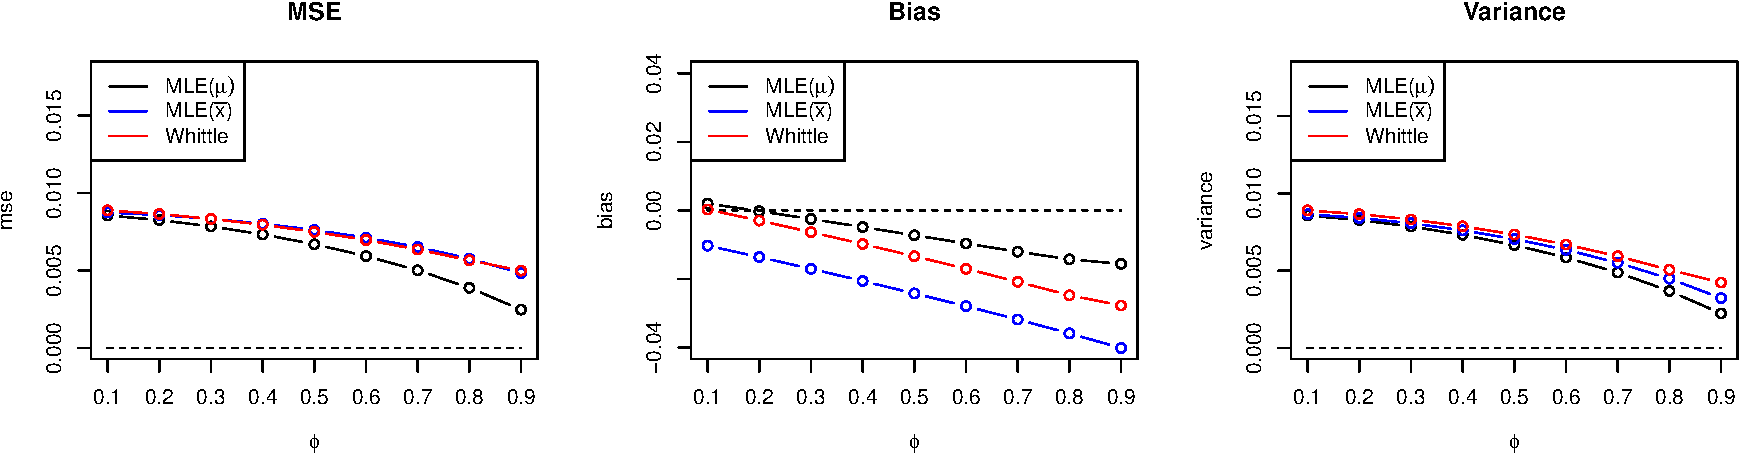
\includegraphics[width=\textwidth]{img/ar1_est_N100.pdf}
		\caption{$n=100$}
	\end{subfigure}
	\begin{subfigure}{\textwidth}
		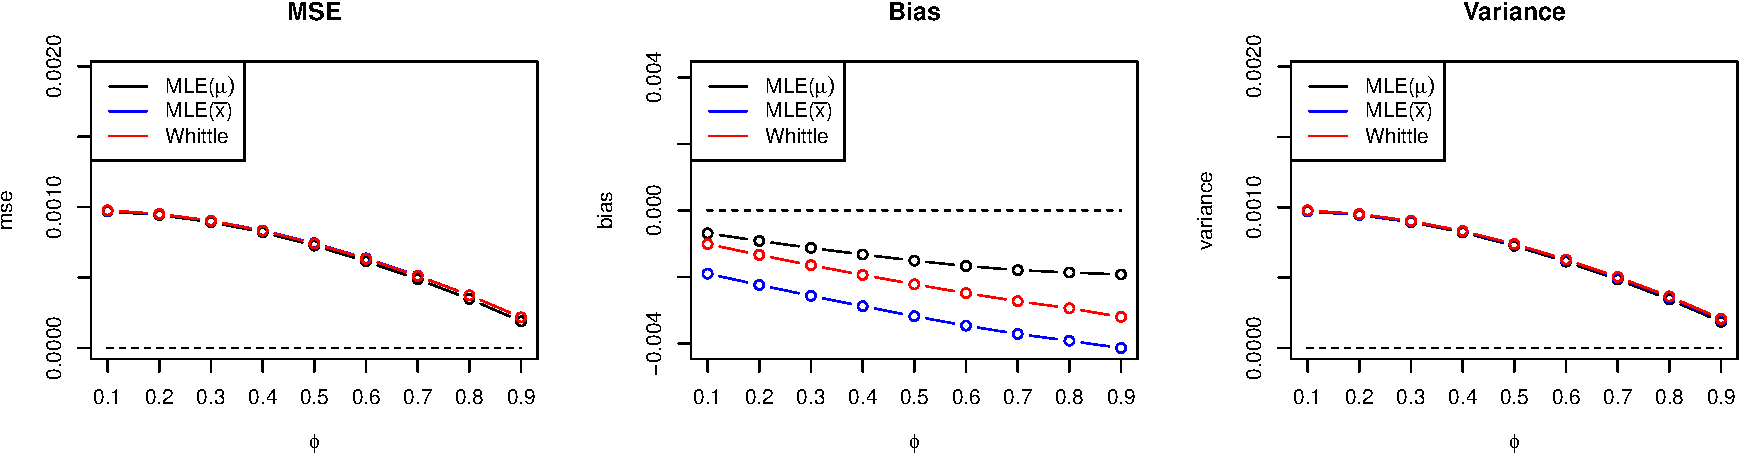
\includegraphics[width=\textwidth]{img/ar1_est_N1000.pdf}
		\caption{$n=1000$}
	\end{subfigure}
	\caption{Среднеквадратичное отклонение, смещение и дисперсия оценок параметра $\phi$ модели $\mathrm{AR}(1)$ ($500$ повторений)}
	\label{fig:ar1_est}
\end{figure}
\begin{figure}[h]
	\centering
	\begin{subfigure}{\textwidth}
		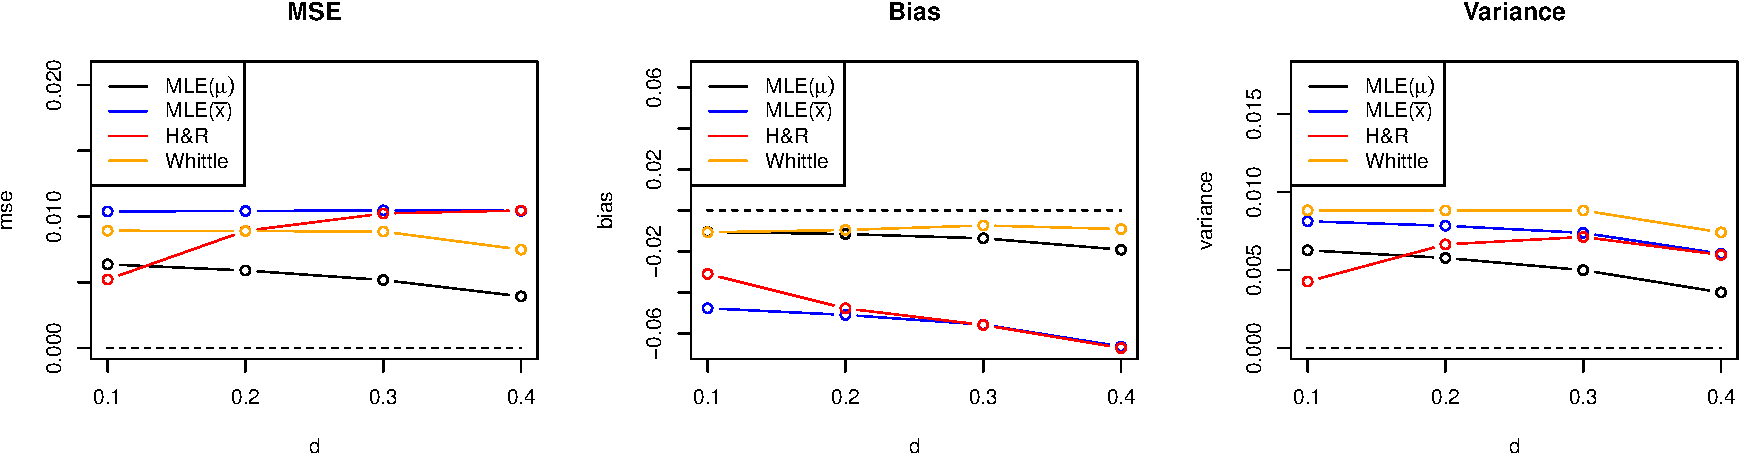
\includegraphics[width=\textwidth]{img/fi_est_N100.pdf}
		\caption{$n=100$}
	\end{subfigure}
	\begin{subfigure}{\textwidth}
		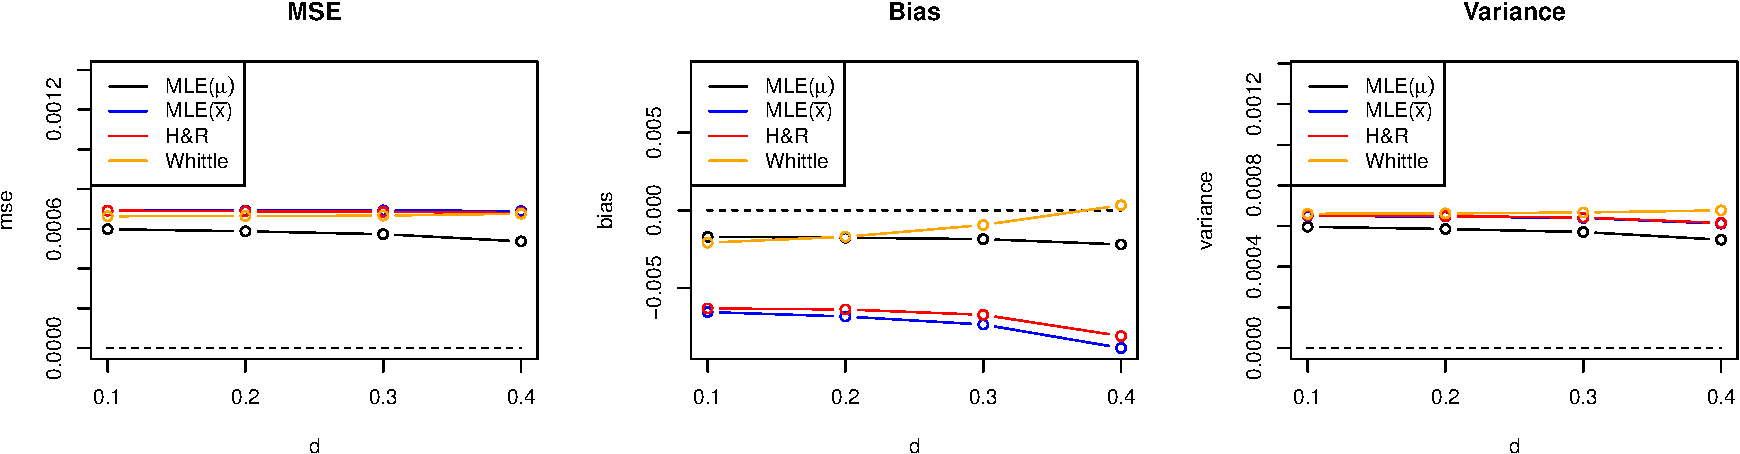
\includegraphics[width=\textwidth]{img/fi_est_N1000.pdf}
		\caption{$n=1000$}
	\end{subfigure}
	\caption{Среднеквадратичное отклонение, смещение и дисперсия оценок параметра $d$ модели $\mathrm{ARFIMA}(0, d, 0)$ ($500$ повторений)}
	\label{fig:fi_est}
\end{figure}

На рис.~\ref{fig:ar1_est} и~\ref{fig:fi_est} изображены среднеквадратичное отклонение, смещение и дисперсия оценок параметров $\phi$ и $d$ моделей $\mathrm{AR}(1)$ и $\mathrm{ARFIMA}(0, d, 0)$. Отметим, что все оценки имеют в большинстве своем отрицательное смещение и отличаются между собой в основном степенью смещения. Как и ожидалось, оценка параметров методом максимального правдоподобия с известным средним дает оценку с наименьшим $\mathsf{MSE}$. С другой стороны, если использовать вместо известного среднего выборочное сренее, оценки становятся сильно смещенными. Whittle же, в свою очередь, дает менее смещенную оценку, чем $\mathrm{MLE}(\bar x)$, а в случае оценки $d$ имеет смещение даже меньше, чем у $\mathrm{MLE}(\mu)$. Однако оценки Whittle обладают наибольшей дисперсией среди всех рассмотренных методов, но разница не такая значительная, как в случае смещения.

\begin{sidewaystable}[h!]
	\centering
	\caption{Смещение и среднеквадратичное отклонение оценок параметров $d$ и $\phi$ модели $\mathrm{ARFIMA}(1, d, 0)$ ($n=100$, $500$ повторений)}
	\label{tab:arfi_est_n100}
	\scalebox{0.9}{
		\begin{tabular}{m{1cm}m{1cm}ccccccccm{0.2cm}cccccccc}
			\hline
			    &        & \multicolumn{8}{c}{$\mathsf{MSE}$}      &                                            & \multicolumn{8}{c}{$\mathsf{Bias}$}                                                                                                                                                                                                                                                                                                                                                                                                              \\
			\cline{3-10} \cline{12-19}
			    &        & \multicolumn{2}{c}{$\mathrm{MLE}(\mu)$} & \multicolumn{2}{c}{$\mathrm{MLE}(\bar x)$} & \multicolumn{2}{c}{H\&R}            & \multicolumn{2}{c}{Whittle} &                         & \multicolumn{2}{c}{$\mathrm{MLE}(\mu)$} & \multicolumn{2}{c}{$\mathrm{MLE}(\bar x)$} & \multicolumn{2}{c}{H\&R} & \multicolumn{2}{c}{Whittle}                                                                                                                                                                                                      \\
			$d$ & $\phi$ & $\hat d$                                & $\hat\phi$                                 & $\hat d$                            & $\hat\phi$                  & $\hat d$                & $\hat\phi$                              & $\hat d$                                   & $\hat\phi$               &                             & $\hat d$                 & $\hat\phi$             & $\hat d$                 & $\hat\phi$ & $\hat d$                 & $\hat\phi$              & $\hat d$                 & $\hat\phi$             \\ \hline
			0.1 & 0.1 & 0.049 & 0.056 & 0.119 & 0.114 & \textcolor{blue}{0.009} & \textcolor{red}{0.018} & 0.069 & 0.067 & & -0.077 & 0.066 & -0.229 & 0.199 & \textcolor{blue}{-0.054} & \textcolor{red}{0.035} & -0.086 & 0.068 \\
			0.2 & 0.1 & 0.047 & 0.055 & 0.151 & 0.141 & \textcolor{blue}{0.025} & \textcolor{red}{0.032} & 0.077 & 0.073 & & \textcolor{blue}{-0.078} & \textcolor{red}{0.067} & -0.265 & 0.232 & -0.119 & 0.099 & -0.094 & 0.074 \\ 
			0.3 & 0.1 & \textcolor{blue}{0.041} & \textcolor{red}{0.049} & 0.183 & 0.165 & 0.049 & 0.055 & 0.084 & 0.081 & & \textcolor{blue}{-0.076} & \textcolor{red}{0.066} & -0.301 & 0.266 & -0.179 & 0.161 & -0.109 & 0.09 \\ 
			0.4 & 0.1 & \textcolor{blue}{0.029} & \textcolor{red}{0.038} & 0.211 & 0.187 & 0.081 & 0.089 & 0.179 & 0.194 & & \textcolor{blue}{-0.072} & \textcolor{red}{0.065} & -0.34 & 0.305 & -0.243 & 0.23 & -0.26 & 0.241 \\ 
			\hline
			0.1 & 0.5 & 0.045 & 0.041 & 0.086 & 0.053 & \textcolor{blue}{0.010} & \textcolor{red}{0.015} & 0.057 & 0.054 & & -0.071 & 0.034 & -0.222 & 0.151 & -0.07 & 0.034 & \textcolor{blue}{-0.066} & \textcolor{red}{0.024} \\ 
			0.2 & 0.5 & 0.042 & 0.038 & 0.092 & 0.055 & \textcolor{blue}{0.031} & \textcolor{red}{0.025} & 0.074 & 0.058 & & \textcolor{blue}{-0.081} & \textcolor{red}{0.046} & -0.244 & 0.171 & -0.154 & 0.108 & -0.153 & 0.107 \\ 
			0.3 & 0.5 & \textcolor{blue}{0.040} & \textcolor{red}{0.036} & 0.1 & 0.059 & 0.063 & 0.043 & 0.098 & 0.062 & & \textcolor{blue}{-0.093} & \textcolor{red}{0.060} & -0.267 & 0.192 & -0.232 & 0.174 & -0.209 & 0.161 \\ 
			0.4 & 0.5 & \textcolor{blue}{0.037} & \textcolor{red}{0.033} & 0.115 & 0.067 & 0.104 & 0.065 & 0.104 & 0.066 & & \textcolor{blue}{-0.103} & \textcolor{red}{0.073} & -0.304 & 0.226 & -0.306 & 0.235 & -0.228 & 0.177 \\
			\hline
			0.1 & 0.9 & 0.029 & 0.029 & 0.014 & 0.01 & \textcolor{blue}{0.007} & \textcolor{red}{0.007} & 0.034 & 0.025 & & 0.075 & -0.089 & 0.01 & -0.049 & \textcolor{blue}{0.001} & \textcolor{red}{-0.043} & 0.049 & -0.069 \\ 
			0.2 & 0.9 & 0.019 & 0.018 & 0.011 & 0.006 & \textcolor{blue}{0.009} & \textcolor{red}{0.004} & 0.026 & 0.019 & & 0.046 & -0.065 & \textcolor{blue}{-0.011} & -0.035 & -0.037 & \textcolor{red}{-0.026} & 0.02 & -0.056 \\ 
			0.3 & 0.9 & 0.012 & 0.01 & \textcolor{blue}{0.009} & 0.004 & 0.014 & \textcolor{red}{0.003} & 0.022 & 0.015 & & \textcolor{blue}{0.016} & -0.043 & -0.033 & -0.023 & -0.076 & \textcolor{red}{-0.011} & -0.024 & -0.039 \\ 
			0.4 & 0.9 & \textcolor{blue}{0.008} & 0.006 & 0.009 & \textcolor{red}{0.002} & 0.025 & \textcolor{red}{0.002} & 0.028 & 0.01 & & \textcolor{blue}{-0.016} & -0.024 & -0.061 & -0.008 & -0.121 & \textcolor{red}{0.003} & -0.095 & -0.016 \\ \hline
		\end{tabular}
	}
\end{sidewaystable}

\begin{sidewaystable}[h!]
	\centering
	\caption{Смещение и среднеквадратичное отклонение оценок параметров $d$ и $\phi$ модели $\mathrm{ARFIMA}(1, d, 0)$ ($n=1000$, $500$ повторений)}
	\label{tab:arfi_est_n1000}
	\scalebox{0.9}{
		\begin{tabular}{m{1cm}m{1cm}ccccccccm{0.2cm}cccccccc}
			\hline
			    &        & \multicolumn{8}{c}{$\mathsf{MSE} \cdot 100$}      &                                            & \multicolumn{8}{c}{$\mathsf{Bias} \cdot 100$}                                                                                                                                                                                                                                                                                                                                                                                                              \\
			\cline{3-10} \cline{12-19}
			    &        & \multicolumn{2}{c}{$\mathrm{MLE}(\mu)$} & \multicolumn{2}{c}{$\mathrm{MLE}(\bar x)$} & \multicolumn{2}{c}{H\&R}            & \multicolumn{2}{c}{Whittle} &                         & \multicolumn{2}{c}{$\mathrm{MLE}(\mu)$} & \multicolumn{2}{c}{$\mathrm{MLE}(\bar x)$} & \multicolumn{2}{c}{H\&R} & \multicolumn{2}{c}{Whittle}                                                                                                                                                                                                      \\
			$d$ & $\phi$ & $\hat d$                                & $\hat\phi$                                 & $\hat d$                            & $\hat\phi$                  & $\hat d$                & $\hat\phi$                              & $\hat d$                                   & $\hat\phi$               &                             & $\hat d$                 & $\hat\phi$             & $\hat d$                 & $\hat\phi$ & $\hat d$                 & $\hat\phi$              & $\hat d$                 & $\hat\phi$             \\ \hline
			0.1 & 0.1 & \textcolor{blue}{0.186} & \textcolor{red}{0.290} & 0.27 & 0.37 & 0.224 & 0.317 & 0.232 & 0.33 & & \textcolor{blue}{-0.581} & \textcolor{red}{0.448} & -1.941 & 1.732 & -1.729 & 1.508 & -0.687 & 0.519 \\ 
            0.2 & 0.1 & \textcolor{blue}{0.181} & \textcolor{red}{0.287} & 0.271 & 0.371 & 0.267 & 0.366 & 0.232 & 0.329 & & \textcolor{blue}{-0.599} & \textcolor{red}{0.465} & -2.026 & 1.824 & -1.981 & 1.773 & -0.615 & 0.468 \\ 
            0.3 & 0.1 & \textcolor{blue}{0.174} & \textcolor{red}{0.282} & 0.272 & 0.372 & 0.268 & 0.367 & 0.232 & 0.328 & & -0.639 & 0.505 & -2.177 & 1.987 & -2.176 & 1.975 & \textcolor{blue}{-0.476} & \textcolor{red}{0.372} \\ 
            0.4 & 0.1 & \textcolor{blue}{0.156} & \textcolor{red}{0.267} & 0.272 & 0.373 & 0.274 & 0.371 & 0.232 & 0.325 & & -0.795 & 0.666 & -2.606 & 2.443 & -2.725 & 2.542 & \textcolor{blue}{-0.263} & \textcolor{blue}{0.233} \\ 
			\hline
			0.1 & 0.1 & 0.761 & 0.8 & 1.429 & 1.3 & \textcolor{blue}{0.504} & \textcolor{red}{0.552} & 1.104 & 1.05 & & \textcolor{blue}{-2.047} & \textcolor{red}{1.588} & -5.86 & 5.102 & -3.256 & 2.741 & -2.555 & 1.904 \\ 
			0.2 & 0.1 & \textcolor{blue}{0.710} & \textcolor{red}{0.759} & 1.432 & 1.302 & 0.978 & 0.969 & 1.213 & 1.125 & & \textcolor{blue}{-2.018} & \textcolor{red}{1.571} & -6.08 & 5.337 & -5.157 & 4.556 & -2.721 & 2.065 \\ 
			0.3 & 0.1 & \textcolor{blue}{0.617} & \textcolor{red}{0.675} & 1.462 & 1.323 & 1.246 & 1.175 & 1.23 & 1.15 & & \textcolor{blue}{-1.984} & \textcolor{red}{1.560} & -6.506 & 5.78 & -6.129 & 5.463 & -2.578 & 1.948 \\ 
			0.4 & 0.1 & \textcolor{blue}{0.473} & \textcolor{red}{0.539} & 1.499 & 1.353 & 1.507 & 1.354 & 1.294 & 1.18 & & \textcolor{blue}{-2.226} & \textcolor{red}{1.861} & -7.514 & 6.838 & -7.622 & 6.905 & -2.695 & 2.099 \\ 
			\hline
			0.1 & 0.9 & 0.338 & 0.155 & 0.288 & 0.122 & \textcolor{blue}{0.259} & \textcolor{red}{0.097} & 0.387 & 0.193 & & 0.623 & -0.774 & \textcolor{blue}{-0.095} & -0.56 & -0.176 & \textcolor{red}{-0.504} & 0.583 & -0.92 \\ 
			0.2 & 0.9 & 0.273 & 0.106 & \textcolor{blue}{0.233} & \textcolor{red}{0.077} & 0.239 & 0.077 & 0.326 & 0.128 & & 0.42 & -0.611 & -0.388 & -0.355 & -0.627 & \textcolor{red}{-0.303} & \textcolor{blue}{0.041} & -0.652 \\ 
			0.3 & 0.9 & 0.241 & 0.093 & \textcolor{blue}{0.217} & \textcolor{red}{0.068} & 0.268 & 0.075 & 0.326 & 0.097 & & \textcolor{blue}{0.287} & -0.53 & -0.667 & -0.204 & -1.395 & \textcolor{red}{-0.029} & -1.003 & -0.285 \\ 
			0.4 & 0.9 & \textcolor{blue}{0.173} & 0.067 & 0.182 & \textcolor{red}{0.051} & 0.381 & 0.076 & 0.545 & 0.09 & & \textcolor{blue}{-0.129} & -0.295 & -1.4 & \textcolor{red}{0.178} & -2.602 & 0.359 & -3.357 & 0.389 \\ 
			\hline
		\end{tabular}
	}
\end{sidewaystable}

В таблицах~\ref{tab:arfi_est_n100} и~\ref{tab:arfi_est_n1000} представлены значения среднеквадратичной ошибки и смещения оценок параметров $d$ и $\phi$ модели $\mathrm{ARFIMA}(1, d)$. Заметим, что в оценках присутствует смещение, для $\phi=0.1$ и $\phi=0.5$ оценки $d$ имеют отрицательное смещение, а оценки $\phi$, наоборот, положительное. Также в таблицах синим цветом выделена лучшая по строке оценка $d$, а красным~--- лучшая оценка $\phi$. Видно, что в случае коротких рядов ($n=100$) метод H\&R в большинстве случаев дает оценки с наименьшим $\mathsf{MSE}$, однако наименьшее смещение имеют оценки $\mathrm{MLE}(\mu)$. В случае же длинных рядов ($n=1000$) наименьшую среднеквадратичную ошибку и смещение дает $\mathrm{MLE}(\mu)$. Отметим, что даже для длинных рядов оценки $\mathrm{MLE}(\bar x)$ имеют, в большинстве случаев, наибольшее смещение и $\mathsf{MSE}$. Оценки H\&R, хотя и дают наименьшее после $\mathrm{MLE}(\mu)$ $\mathsf{MSE}$, также сильно смещены. Оценки методом Whittle выглядят наиболее привлекательными, поскольку имеют наименьшее после $\mathrm{MLE}(\mu)$ смещение и имеют $\mathsf{MSE}$ меньше, чем $\mathrm{MLE}(\bar x)$.

Подведем итоги численнного сравнения. Если для рассматриваемого ряда известно его матожидание $\mu$ (что, конечно, редкость на практике), наилучшим методом является $\mathrm{MLE}(\mu)$. Если же среднее неизвестно, для коротких рядов оценивать параметры моделей $\mathrm{AR}(1)$ и $\mathrm{ARFIMA}(0, d, 0)$ следует методом Whittle, а параметры модели $\mathrm{ARFIMA}(1, d, 0)$~--- методом H\&R. В случае длинных рядов параметры рассматриваемых моделей следует оценивать методом Whittle.

% \begin{table}[h!]
% 	\centering
% 	\caption{Смещение и среднеквадратичное отклонение оценок параметра $\phi$ модели $\mathrm{AR}(1)$ ($n=100$, $500$ повторений)}
% 	\begin{tabular}{m{1cm}cccm{0.5cm}ccc}
% 		\hline
% 		& \multicolumn{3}{c}{$\mathsf{bias}\cdot 100$} & & \multicolumn{3}{c}{$\mathsf{MSE}\cdot 100$} \\
% 		\cline{2-4} \cline{6-8}
% 		$\phi$ & $\mathrm{MLE}(\mu)$ & $\mathrm{MLE}(\bar x)$ & Whittle & & $\mathrm{MLE}(\mu)$ & $\mathrm{MLE}(\bar x)$ & Whittle \\ \hline
% 		0.1 & 0.197  & -1.029 &  0.025 & & 0.856 & 0.874 & 0.889\\
% 		0.2 & -0.023 & -1.362 & -0.298 & & 0.826 & 0.859 & 0.865\\
% 		0.3 & -0.252 & -1.707 & -0.635 & & 0.785 & 0.834 & 0.834\\
% 		0.4 & -0.487 & -2.061 & -0.981 & & 0.733 & 0.802 & 0.796\\
% 		0.5 & -0.725 & -2.423 & -1.337 & & 0.670 & 0.762 & 0.75\\
% 		0.6 & -0.965 & -2.796 & -1.704 & & 0.594 & 0.712 & 0.697\\
% 		0.7 & -1.205 & -3.183 & -2.084 & & 0.502 & 0.652 & 0.636\\
% 		0.8 & -1.427 & -3.59  & -2.478 & & 0.389 & 0.577 & 0.566\\
% 		0.9 & -1.560 & -4.016 & -2.777 & & 0.248 & 0.483 & 0.5\\
% 		\hline
% 	\end{tabular}
% \end{table}

\subsection{Сходимость оценок к истинным значениям}
Известно~\cite[Theorem 8.1]{Hassler2018}, что
\begin{equation}\label{eq:mle_distribution}
	\sqrt{n}(\widehat{\bm\varphi}_\mathrm{ML} - \bm\varphi_0)\overset{d}{\longrightarrow} \mathcal{N}_{k+1}(0, \mathcal{I}^{-1}(\bm{\varphi}_0)),
\end{equation}
где $\bm\varphi_0$~--- истинный вектор параметров, $\mathcal{I}(\bm\varphi)$~--- информационная матрица Фишера. Также известно~\cite[Proposition 8.3]{Hassler2018}, что вектор $\widehat{\bm\varphi}_W$ имеет такое же асимптотическое распределение, что и $\widehat{\bm\varphi}_\mathrm{ML}$.

Покажем, что методы $\mathrm{MLE}(\mu)$ и Whittle реализованы корректно, посмотрев на дисперсию оценок для $n=10000$. В таблице~\ref{tab:variance} представлены оценки дисперсий $\hat d$ и $\hat \phi$, в скобках указана теоретическая дисперсия. Как видим, для разных значений параметров значение дисперсий оценок близки к теоретическим.

\begin{table}[h]
	\centering
	\subfloat[$d=0.2$, $\varphi=0.1$]{
		\begin{tabular}{c|cc}
			Метод & $n\mathsf{D} \hat d$ (1.83167) & $n\mathsf{D}\hat \phi$ (2.98284) \\
			\hline
			$\mathrm{MLE}(\mu)$ & 1.72733 & 2.92604 \\
			Whittle & 1.78350 & 2.94929 \\
			\hline
		\end{tabular}
	}
	\subfloat[$d=0.4$, $\varphi=0.1$]{
			\begin{tabular}{c|cc}
				Метод & $n\mathsf{D} \hat d$ (1.83167) & $n\mathsf{D}\hat \phi$ (2.98284) \\
				\hline
				$\mathrm{MLE}(\mu)$ & 1.69348 & 2.90374 \\
				Whittle & 1.84265 & 2.96828 \\
				\hline
			\end{tabular}
	}\vspace{2em}
	\subfloat[$d=0.2$, $\varphi=0.5$]{
		\begin{tabular}{c|cc}
			Метод & $n\mathsf{D} \hat d$ (4.91219) & $n\mathsf{D}\hat \phi$ (6.06018) \\
			\hline
			$\mathrm{MLE}(\mu)$ & 5.00869 & 6.305 \\
			Whittle & 5.08405 & 6.35985 \\
			\hline
		\end{tabular}
	}
	\subfloat[$d=0.4$, $\varphi=0.5$]{
		\begin{tabular}{c|cc}
			Метод & $n\mathsf{D} \hat d$ (4.91219) & $n\mathsf{D}\hat \phi$ (6.06018) \\
			\hline
			$\mathrm{MLE}(\mu)$ & 4.75975 & 6.06711 \\
			Whittle & 5.28104 & 6.4936 \\
			\hline
		\end{tabular}
	}\vspace{2em}
	\subfloat[$d=0.2$, $\varphi=0.9$]{
		\begin{tabular}{c|cc}
			Метод & $n \mathsf{D} \hat d$ (2.49203) & $n\mathsf{D}\hat \phi$ (0.77885) \\
			\hline
			$\mathrm{MLE}(\mu)$ & 2.42011 & 0.78209 \\
			Whittle & 2.44394 & 0.77549 \\
			\hline
		\end{tabular}
	}
	\subfloat[$d=0.4$, $\varphi=0.9$]{
		\begin{tabular}{c|cc}
			Метод & $n \mathsf{D} \hat d$ (2.49203) & $n\mathsf{D}\hat \phi$ (0.77885) \\
			\hline
			$\mathrm{MLE}(\mu)$ & 2.26718 & 0.749318  \\
			Whittle & 2.57117 & 0.77311 \\
			\hline
		\end{tabular}
	}
	\caption{Дисперсия оценок $\hat d$ и $\hat \phi$, $n=10000$, $100$ повторений}
	\label{tab:variance}
\end{table}

\chapter{Метод Monte Carlo SSA}\label{chpt:mcssa}
\section{Проверка статистических гипотез}
Рассмотрим некоторый критерий со статистикой $T$. Введем обозначения.
% \begin{definition}
% 	p-value~--- такое значение $\mathrm p$, что при значениях уровня значимости $\alpha$, больших $\mathrm p$, $H_0$ отвергается (статистика попадает в критическую область $A_\text{крит}(\alpha)$), а при меньших~--- не отвергается.
% \end{definition}
\begin{definition}
	Ошибка первого рода~--- вероятность отвергнуть нулевую гипотезу, если она верна: $\alpha_I(\alpha)=\mathsf P_{H_0}(T\in A_\text{крит}(\alpha))$.
\end{definition}
\begin{definition}
	Если $\alpha_I=\alpha$, то говорят, что критерий точный при уровне значимости $\alpha$, иначе говорят, что критерий неточный. При $\alpha_I<\alpha$ критерий является консервативным, а при $\alpha_I>\alpha$~--- радикальным.
\end{definition}
\begin{definition}
	Мощность критерия против альтернативы $H_1$~--- вероятность отвергнуть нулевую гипотезу, если верна альтернативная: $\beta(\alpha)=\mathsf P_{H_1}(T\in A_\text{крит}(\alpha))$.
\end{definition}
% \begin{remark}
% 	По определению p-value $\alpha_I(\alpha)=\mathsf P_{H_0}(\mathrm p < \alpha)$ и $\beta(\alpha)=\mathsf P_{H_1}(\mathrm p < \alpha)$.
% \end{remark}

\subsection{Поправка неточных критериев}\label{sect:correction}
Зафиксируем некоторый неточный (консервативный или радикальный) критерий и уровень значимости $\alpha^*$. Пусть дана зависимость ошибки первого рода от уровня значимости $\alpha_I(\alpha)=\mathsf P_{H_0}(\mathrm p < \alpha)$. Тогда критерий с формальным уровнем значимости $\widetilde\alpha^*=\alpha_I^{-1}(\alpha^*)$ является точным: ошибка первого рода $\alpha_I(\widetilde\alpha^*)=\alpha^*$.

Если зависимость $\alpha_I(\alpha)$ неизвестна, она оценивается с помощью моделирования. Приведем алгоритм поправки в этом случае. Помимо критерия и уровня значимости, зафиксируем количество выборок $M$ для оценки $\alpha_I(\alpha)$ и их объем $N$.
\begin{algorithm}{Поправка уровня значимости по зависимости $\alpha_I(\alpha)$}~\cite{Larin2022}\label{alg:correction}
	\begin{enumerate}
		\item Моделируется $M$ выборок объема $N$ при верной $H_0$.
		\item По моделированным данным строится оценка зависимость ошибки первого рода от уровня значимости $\alpha_I(\alpha)$.
		\item Рассчитывается формальный уровень значимости: $\widetilde{\alpha}^*=\alpha_I^{-1}(\alpha^*)$. Критерий с таким уровнем значимости является асимптотически точным при $M\to\infty$.
	\end{enumerate}
\end{algorithm}

\subsection{Сравнение критериев}
Точные критерии, проверяющие одну и ту же гипотезу, можно использовать и сравнивать по мощности: чем больше мощность, тем лучше. Если критерий является консервативным, использовать и сравнивать его с другими критерии по мощности также можно, учитывая, что его мощность будет занижена. Радикальный же критерий, без поправки, введенной в разделе~\ref{sect:correction}, нельзя использовать и сравнивать по мощности с другими критериями. Поэтому введем понятие ROC-кривой, соответствующее мощности критерия, к которому была применена поправка.
\begin{definition}
	ROC-кривая~--- это кривая, задаваемая параметрически
	\[
		\begin{cases}
			x=\alpha_I(\alpha) \\
			y=\beta(\alpha)
		\end{cases},\quad \alpha\in[0,1]
	\]
\end{definition}
\begin{remark}
	С помощью ROC-кривых можно сравнивать по мощности неточные (в частности, радикальные) критерии. Отметим, что для точного критерия ROC-кривая совпадает с графиком мощности, так как $\alpha_I(\alpha)=\alpha$.
\end{remark}

\section{Monte Carlo SSA}
Метод Monte Carlo SSA (MC-SSA) тестно связан с методом SSA (Singular Spectrum Analysis), стостоящим из четырех этапов: \emph{вложения}, \emph{разложения}, \emph{группировки} и \emph{диагонального усреднения}. Поэтому опишем сначала его.
\subsection{Метод SSA}
Пусть $\tX=(x_1,\ldots,x_N)$~--- временной ряд длины $N$. Зафиксируем длину окна $L$, $1<L<N$. Рассмотрим $K=N-L+1$ векторов вложения $X_i=(x_i,\ldots,x_{i+L-1})$ и составим из столбцов $X_i$ так называемую траекторную матрицу:
\[
	\bfX = [X_1:\ldots:X_K].
\]
Далее траекторная матрица $\bfX$ разбивается в сумму матриц единичного ранга. В базовом SSA используются собственные векторы матрицы $\bfX\bfX^\rmT$, в Toeplitz SSA используются собственные векторы матрицы $\bfT$ с элементами
\begin{equation}\label{eq:toeplitz}
	t_{ij} = \frac{1}{N - |i - j|}\sum_{n=1}^{N - |i - j|}x_n x_{n+|i-j|},\quad i,j\leqslant L.
\end{equation}
Обозначим за $P_1,\ldots,P_L$ собственные векторы матрицы $\bfX\bfX^\rmT$ либо матрицы $\bfT$. Тогда получаем следующее разложение:
\[
	\bfX = \sum_{i=1}^L \sigma_i P_i Q_i^\rmT = \bfX_1+\ldots+\bfX_L,
\]
где $S_i=\bfX^\rmT P_i$, $Q_i=S_i/\|S_i\|$, $\sigma_i=\|S_i\|$.

После этого полученные матрицы группируются и каждая из группированных матриц преобразовывается обратно во временной ряд. Таким образом, результатом SSA является разложение временного ряда.
\subsection{Постановка задачи}
Рассмотрим задачу поиска сигнала (неслучайной составляющей) во временном ряде. Модель выглядит следующим образом:
\[
	\tX=\tS + \bm\xi,
\]
где $\tS$~--- сигнал, $\bm\xi$~--- стационарный процесс с нулевым средним. Тогда нулевая гипотеза $H_0:\tS=0$ (отсутствие сигнала, ряд состоит из чистого шума) и альтернатива $H_1:\tS\ne0$ (ряд содержит сигнал, например, периодическую составляющую).
% \begin{definition}
% 	Случайный процесс $\bm\xi=(\xi_1,\dots,\xi_n, \ldots)$ называют красным шумом с параметрами $\varphi$ и $\delta$, если $\xi_n = \varphi\xi_{n-1} + \delta\varepsilon_n$, где $0<\varphi<1$, $\varepsilon_n$~--- белый гауссовский шум с дисперсией 1 и $\xi_1$ имеет нормальное распределение с нулевым средним и дисперсией $\delta^2/(1-\varphi^2)$.
% \end{definition}
% В этой и следующей главах под шумом будем подразумевать именно красный, причем в данной главе с известными параметрами.   Также будем рассматривать только односторонние критерии.

% \subsection{Одиночный тест}\label{sect:single_test}
% Зафиксируем длину окна $L$ и обозначим траекторную матрицу ряда $\bm\xi$ как $\mathbf\Xi$. Рассмотрим вектор $W\in \R^{L}$ такой, что $\|W\|=1$. Введем величину
% \[
% 	p=\|\mathbf{\Xi}^\rmT W\|^2.
% \]
% Статистикой критерия является величина
% \[
% 	\widehat{p}=\|\bfX^\rmT W\|^2.
% \]
% Если вектор $W$~--- синусоида с частотой $\omega$, то $\widehat{p}$ отражает вклад частоты $\omega$ в исходный ряд.

% Рассмотрим алгоритм статистического критерия проверки наличия сигнала в ряде с проекцией на один вектор $W$, описанный в работе~\cite{Golyandina2023}.
% \begin{algorithm}{Одиночный тест~\cite{Golyandina2023}}
% 	\begin{enumerate}
% 		\item Построить статистику критерия $\widehat p$.
% 		\item Построить доверительную область случайной величины $p$: интервал от нуля до $(1-\alpha)$-квантиля, где $\alpha$~--- уровень значимости.
% 		\item Если $\widehat p$	не попадает в построенный интервал~--- $H_0$ отвергается.
% 	\end{enumerate}
% \end{algorithm}
% Построенная доверительная область называется \textit{прогнозируемым интервалом} с уровнем доверия $1-\alpha$.
% \begin{remark}
% В большинстве случаев, распределение $p$ неизвестно. Поэтому оно оценивается методом Монте-Карло: берется $G$ реализаций случайного процесса $\boldsymbol\xi$, для каждой вычисляется $p$ и строится эмпирическое распределение. В связи с этим в названии метода присутствуют слова <<Monte Carlo>>.
% \end{remark}
% \begin{remark}
% Если частота $\omega$ сигнала $\tS$ известна, то в качестве $W$ можно взять синусоиду с частотой $\omega$. Но на практике $\omega$ редко бывает известна, что делает данный критерий несостоятельным против $H_1$.
% \end{remark}

\subsection{Множественный тест}\label{sect:multiple_test}
Зафиксируем длину окна $L$ и модель шума $\bm\xi$. Пусть $\tR_1, \ldots, \tR_G$~--- реализации $\bm\xi$, которые в дальнейшем будем называть суррогатными. Обозначим за $\bfX$ и $\bm\Xi_i$, $i=1,\ldots, G$, траекторные матрицы ряда $\tX$ и каждой суррогатной реализации соответственно. Рассмотрим $H$ проекционных векторов $W_1,\ldots,W_H$, соответствующих некоторой частоте $\omega_k$, $\|W_k\|=1$, $k=1,\ldots,H$.
% Пусть теперь частоты периодических компонент неизвестны, что не редкость на практике. Тогда подобно одиночному тесту рассмотрим набор $W_1,\ldots,W_H$ векторов для проекции, и для каждого $k=1,\ldots,H$ построим статистику критерия $\widehat p_k$:
% \begin{equation}\label{eq:mc-ssa_statisctics}
% 	\widehat p_k = \|\bfX^\rmT W_k\|^2,\quad k=1,\ldots,H.
% \end{equation}
% В таком случае нужно построить $H$ предсказательных интервалов для каждого $W_k$ по выборкам $P_k=\{p_{ki}\}_{i=1}^G$ с элементами
% \begin{equation}\label{eq:mc-ssa_h0}
% 	p_{ki}=\|\mathbf{\Xi}_i^\rmT W_k\|^2,\quad i=1,\ldots,G;\ k=1,\ldots,H,
% \end{equation}
% где $G$~--- количество суррогатных реализаций $\bm\xi$, $\mathbf{\Xi}_i$~--- траекторная матрица $i$-й реализации $\bm\xi$.

% В работе~\cite{Golyandina2023} подробно описана проблема множественного тестирования, когда вероятность ложного обнаружения периодической составляющей для одной из рассматриваемых частот (групповая ошибка I рода) неизвестна и значительно превышает заданный уровень значимости (частота ошибок одиночного теста), и ее решение. Приведем модифицированный алгоритм построения критерия в случае множественного тестирования, который будем использовать в дальнейшем.
\begin{algorithm}{Multiple MC-SSA~\cite{Golyandina2023}}\label{alg:multiple_mc-ssa}
	\begin{enumerate}
		\item Для $k=1,\dots,H$ вычисляется статистика $\widehat{p}_k=\|\bfX^\rmT W_k\|^2$, выборка $P_k=\{p_{ki}\}_{i=1}^G$ с элементами $p_{ki}=\|\bm\Xi_i^\rmT W_k\|^2$, ее среднее $\mu_k$ и стандартное отклонение $\sigma_k$.
		\item Вычисляется $\mathbf{\eta}=(\eta_1,\dots,\eta_G)$, где
		      \[
			      \eta_i=\max_{1\leqslant k\leqslant H}(p_{ki}-\mu_k)/\sigma_k,\quad i=1,\dots,G.
		      \]
		\item Находится $q$ как выборочный $(1-\alpha)$-квантиль $\eta$, где $\alpha$~--- уровень значимости.
		\item Нулевая гипотеза не отвергается, если
		      \[
			      t = \max_{1\leqslant k\leqslant H}(\widehat{p}_k-\mu_k)/\sigma_k<q.
		      \]
		\item Если $H_0$ отвергнута, вклад $W_k$ (и соответствующей частоты) значим, если $\widehat{p}_k$ превосходит $\mu_k+q\sigma_k$. Таким образом, $[0,\mu_k+q\sigma_k]$ считаются скорректированными интервалами прогнозирования.
	\end{enumerate}
\end{algorithm}

\subsection{Ограничение на модель шума}
Для модели модели шума $\bm\xi$ важно, чтобы спектральная плотность процесса была строго монотонной. Это связано с тем, что собственные векторы автоковариационной матрицы стационарного процесса ведут себя как синусоиды с равностоящими частотами, а соответсвующие им собственные числа примерно равны значению спектральной плотности в этих частотах. Тогда при строгой монотонности $f_{\bm\xi}(\omega)$ вклад этих векторов будет попарно различным, делая их сильно разделимыми~\cite[Раздел 1.5.4]{Golyandina2001}. Если же опустить требование строгой монотонности, компоненты могут смешаться, что делает невозможным определение доминирущей частоты значимого вектора.
\begin{remark}
	Примерами процессов со строго монотонной спектральной плотностью являются красный шум и модель $\mathrm{ARFIMA}(0, d, 0)$.
\end{remark}
Для процессов с короткой памятью утверждение о виде собственных чисел и собственных векторов верно, поскольку теплицеву симметричную матрицу можно апроксимировать циркулянтной матрицей~\cite{Gray2005}, собственные векторы которой равны
\[
	v_j=\frac{1}{\sqrt n}\left(1, \omega^j, \omega^{2j},\ldots,\omega^{(n-1)j}\right),\quad j=0,1\ldots,n-1,
\]  
а соответвующие им собственные числа равны
\[
\lambda_j = \sum_{k=0}^{n-1}c_k\omega^{j},
\]
где $\omega=\exp\{2\pi\im / n\}$.

Для процессов с длинной памятью покажем правдивость этого факта, проведя численный эксперимент. Рассмотрим модель $\mathrm{ARFIMA}(0, d, 0)$ с $d=0.4$ и пусть размер автоковариационной матрицы $\bm\Sigma_n$ равен $n=100$. Частоту векторов будем оценивать с помощью метода \textsf{ESPRIT}~\cite[Раздел 3.1]{SSA_R}.

\begin{figure}[h]
	\begin{subfigure}{\textwidth}
		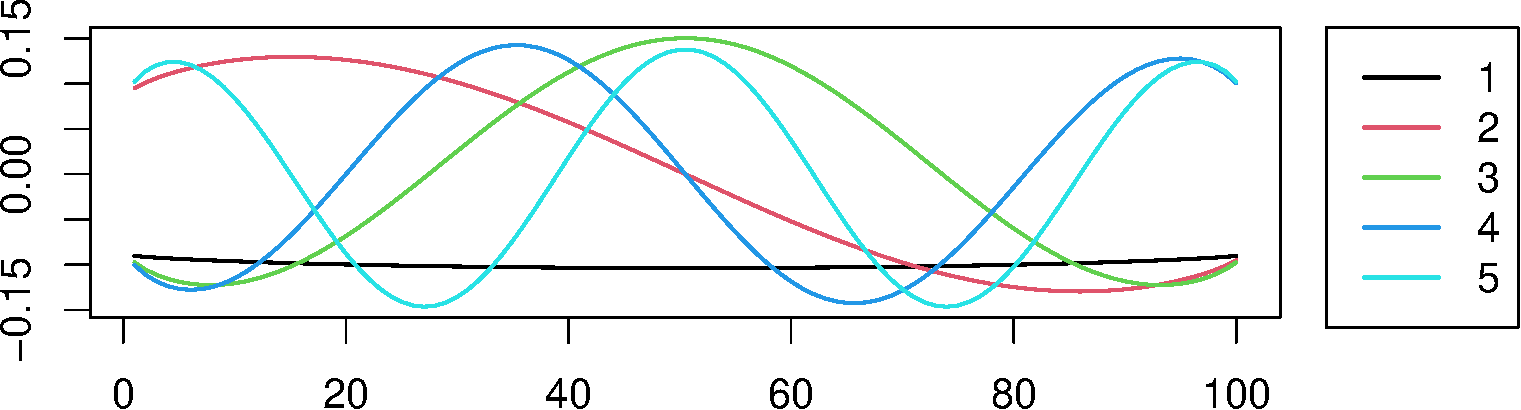
\includegraphics[width=\textwidth]{img/eigenvectors_longmemo1.pdf}
	\end{subfigure}
	\begin{subfigure}{\textwidth}
		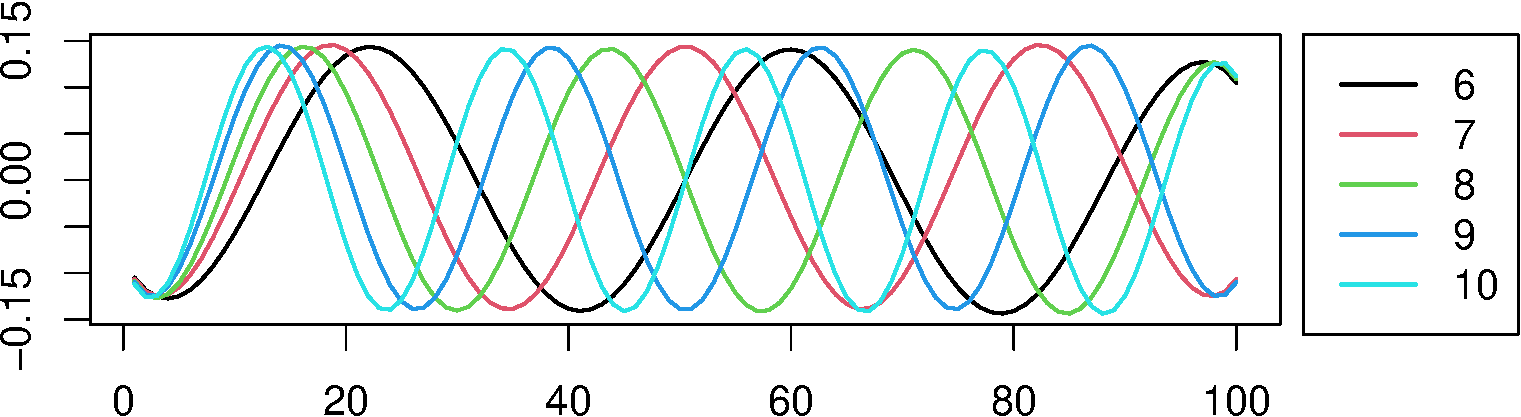
\includegraphics[width=\textwidth]{img/eigenvectors_longmemo2.pdf}
	\end{subfigure}
	\caption{Собственные векторы автоковариационной матрицы модели $\mathrm{ARFIMA}(0, d, 0)$}
	\label{fig:eigenvectors_longmemo}
\end{figure}

\begin{figure}[h]
	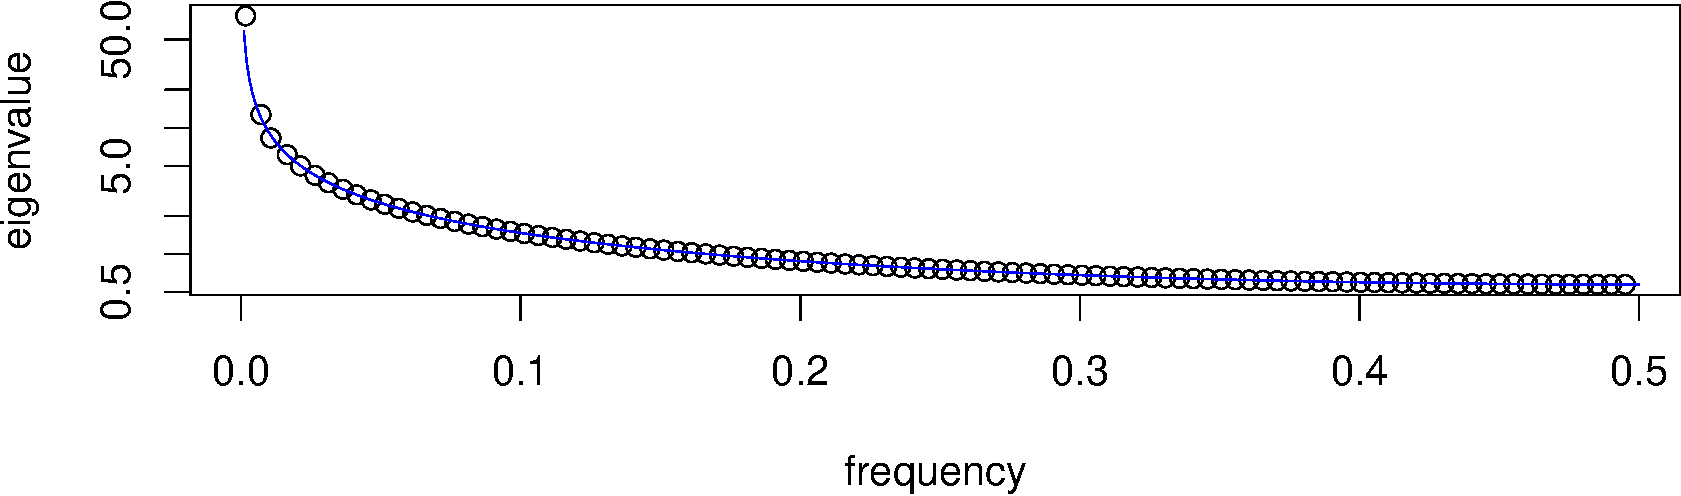
\includegraphics[width=\textwidth]{img/eigenvalues_longmemo.pdf}
	\caption{Собственные числа автоковариационной матрицы модели $\mathrm{ARFIMA}(0, d, 0)$}
	\label{fig:eigenvalues_longmemo}
\end{figure}

\begin{figure}[h]
	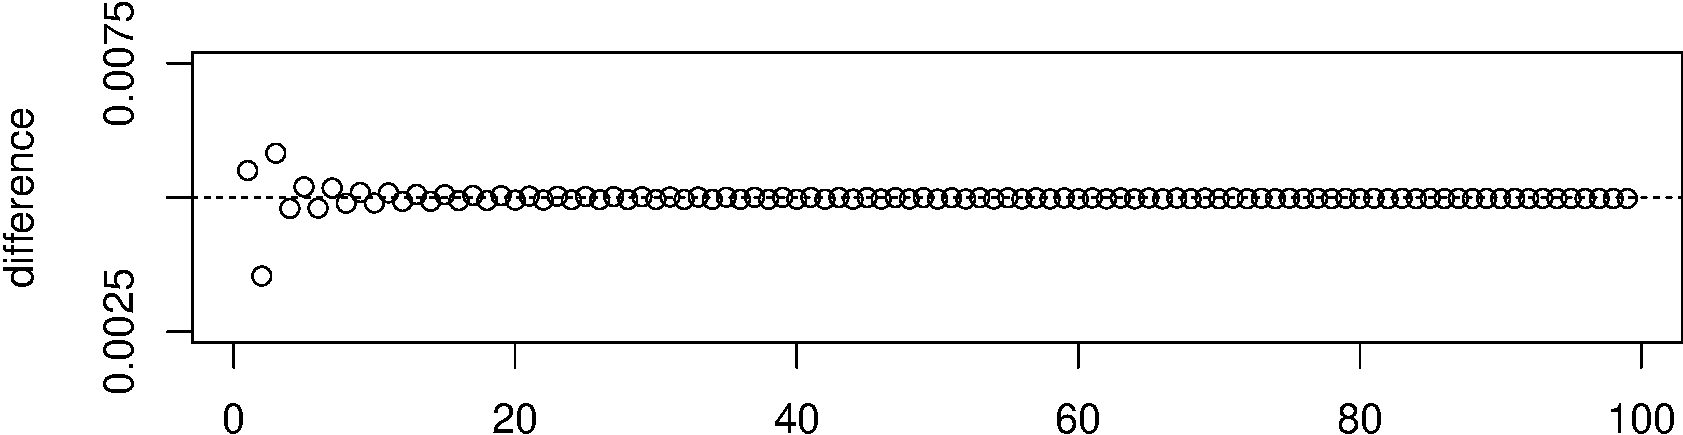
\includegraphics[width=\textwidth]{img/eigenvectors_freq_diff.pdf}
	\caption{Разница частот между ближайшими собственными векторами}
	\label{fig:freq_diff}
\end{figure}

На рис.~\ref{fig:eigenvectors_longmemo} представлены первые $10$ собственных векторов матрицы $\bm\Sigma_n$, на рис.~\ref{fig:eigenvalues_longmemo} по оси $Ox$ отложена частота, которой соответствует собственный вектор, а по оси $Oy$ отложено соответвующее вектору собственное число, дополнительно синей линией проведена спектральная плотность процесса. Как видим, действительно, собственные векторы ведут себя как периодики, собственные числа хорошо приближаются значением спектральной плотности в соответствующей частоте, и по рис.~\ref{fig:freq_diff} разница между частотами примерно равна $1 / (2n)=0.005$.

\subsection{Используемый вариант MC-SSA}\label{sect:vectors_choise}
В разделе~\ref{sect:multiple_test} предполагалось, что векторы $W_1,\ldots, W_H$ фиксированные и не зависят от исходного ряда. Такой критерий MC-SSA является точным, то есть ошибка первого рода равна заданному уровню значимости. В этой работе будут рассматриваться векторы $W_k$, порожденные рядом $\tX$, при этом по-прежнему при вычислении $p_{ki}$ используются те же $W_k$, что и при вычислении $\widehat p_k$.
% \begin{remark}\label{remark:complexity}
% 	Если критерий MC-SSA точный и не требует поправки, то его трудоемкость состоит из трудоемкости одного разложения траекторной матрицы исходного ряда и $G$ вычислений по формуле~\eqref{eq:mc-ssa_h0}. При применении поправки трудоемкость увеличивается в $M$ раз, где $M$~--- количество выборок для оценки зависимости $\alpha_I(\alpha)$.
% \end{remark}

Поскольку в этом варианте векторы $W_k$ не заданы заранее, а порождены исходным рядом, критерий MC-SSA становится, вообще говоря, радикальным. Бороться с этой проблемой позволяет метод эмпирической поправки критерия, описанный в разделе~\ref{sect:correction}.

В качестве $W_1, \ldots,W_H$ будем брать собственные векторы матрицы $\bfX\bfX^\rmT$ или $\bfT$ (см. формулу~\eqref{eq:toeplitz}). Такой способ выбора векторов для проекции самый распространенный, поскольку, если есть значимые векторы, можно восстановить сигнал с помощью SSA на их основе. Будем под MC-SSA подразумевать именно этот вариант критерия. Варианты критерия будут определяться конкретным разложением траекторной матрицы. Заметим, что обычно используется сингулярное разложение.


\subsection{Сравнение MC-SSA по мощности при разных моделях шума}
Пусть $\bm \xi$~--- красный шум, а $\bm \eta$~--- модель $\mathrm{ARFIMA}(0, d, 0)$. Будем считать дисперсию белого шума одинаковой для обоих процессов и равной $\sigma^2$. Дисперсии $\bm\xi$ и $\bm\eta$ соответственно равны
\[
	\mathsf{D}\bm\xi = \frac{\sigma^2}{1 - \phi^2}, \quad \mathsf{D}\bm\eta = \sigma^2\frac{\Gamma(1 - 2d)}{\Gamma(1-d)^2}.
\]
Тогда дисперсии процессов равны тогда и только тогда, когда
\[
	\phi=\pm\sqrt{1-\frac{\Gamma(1-d)^2}{\Gamma(1-2d)}}.
\]

\begin{figure}[h]
	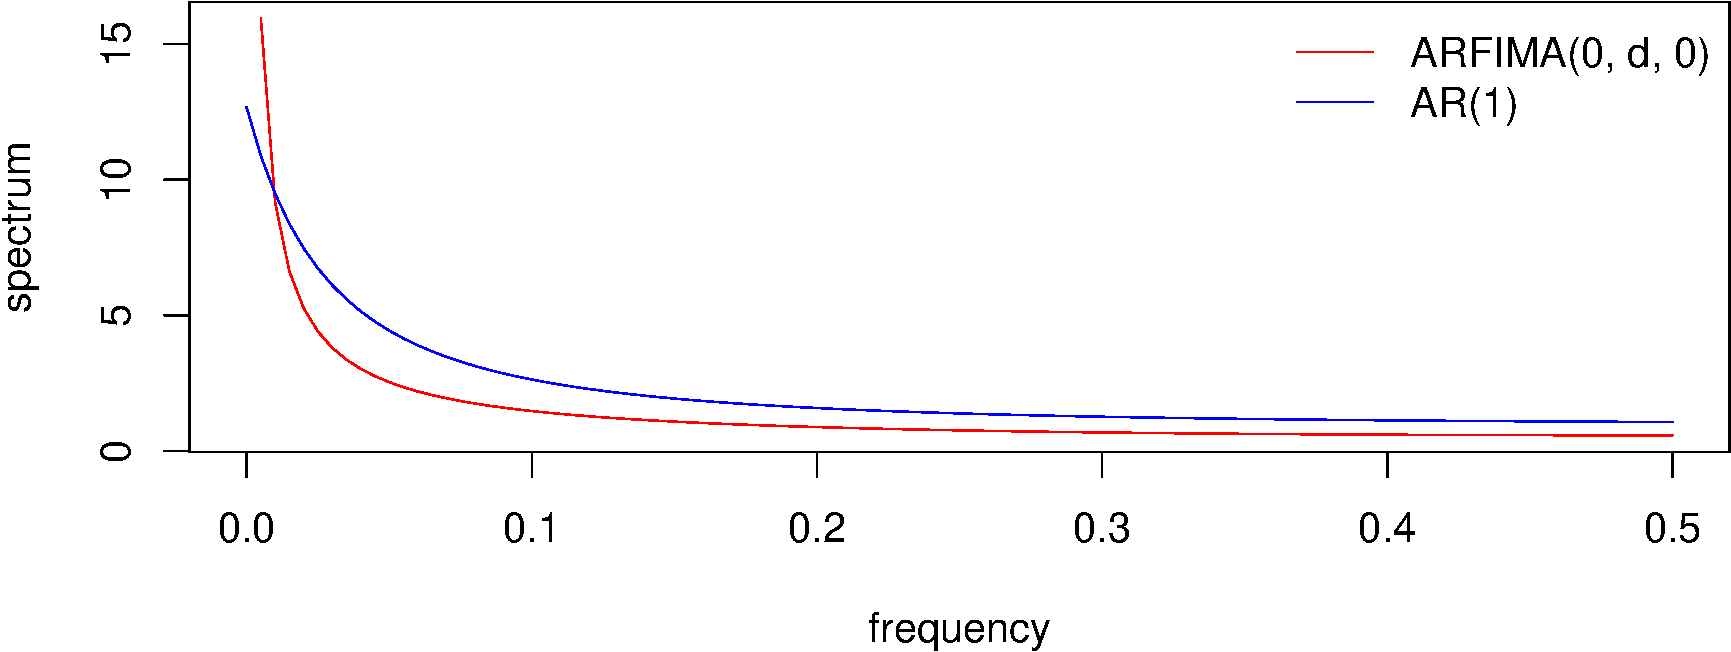
\includegraphics[width=\textwidth]{img/spectrum.pdf}
	\caption{Спектральная плотность процессов с одинаковой дисперсией}
	\label{fig:spectrum}
\end{figure}

Пусть $d=0.4$. Тогда при $\phi\approx0.719$ процессы $\bm\xi$ и $\bm\eta$ имеют одинаковую дисперсию. На рис.~\ref{fig:spectrum} изображены спектральные плотности процессов. На нем видно, что процесс $\bm\eta$ имеет меньшее значение плотности для всех значений $\omega$, за исключением близких к нулю.

Предполагается, что если рассмотреть в качестве альтернативы сигнал с частотой $\omega:f_{\bm\eta}(\omega) < f_{\bm\xi}(\omega)$, то мощность критерия MC-SSA против этой альтереативы при модели шума $\bm\eta$ больше, чем при модели шума $\bm\xi$. Убедимся в этом. Пусть длина ряда $N=100$, $\sigma^2=1$ и
\[
	\tS = \{A\cos(2 \pi n \omega)\}_{n=1}^N,\quad A=1,\ \omega=0.075.
\]
% Тогда $H_0:\tS=0$ и $H_0:\tS\ne0$.

\begin{figure}[h]
	\begin{subfigure}{\textwidth}
		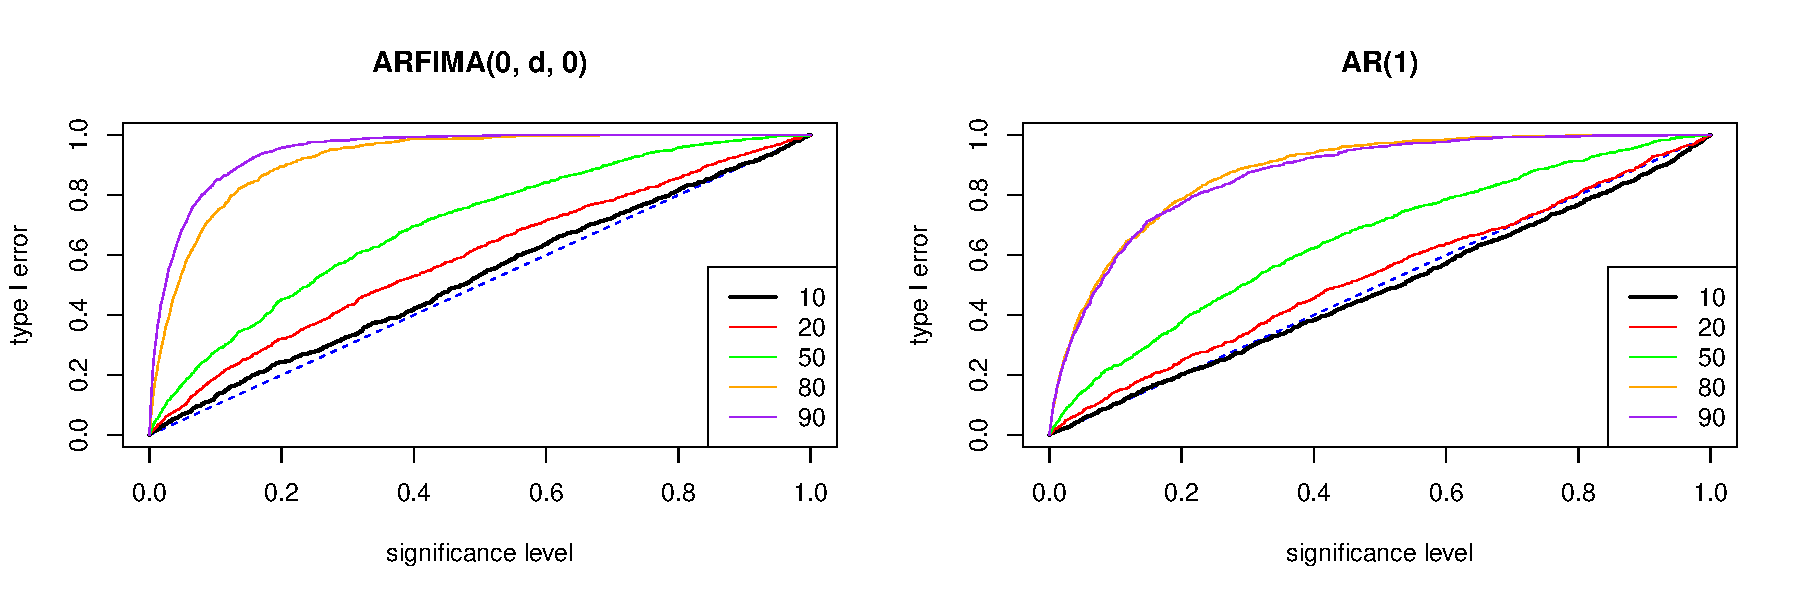
\includegraphics[width=\textwidth]{img/alphaI_comp.pdf}
		\caption{Ошибка первого рода}
		\label{fig:ar1_vs_fi_alphaI}
	\end{subfigure}
	\begin{subfigure}{\textwidth}
		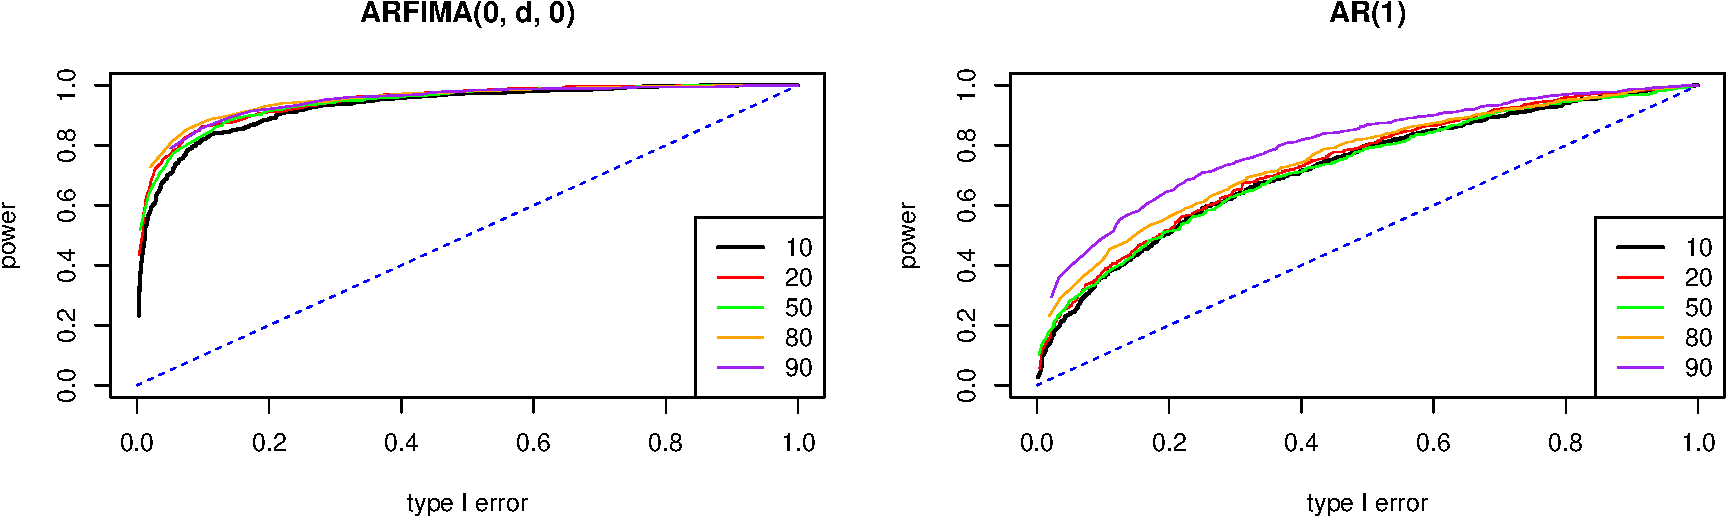
\includegraphics[width=\textwidth]{img/roc_comp.pdf}
		\caption{ROC-кривая}
		\label{fig:ar1_vs_fi_roc}
	\end{subfigure}
	\caption{Сравнение мошностей MC-SSA}
	\label{fig:ar1_vs_fi}
\end{figure}
На рис.~\ref{fig:ar1_vs_fi_alphaI} изображены график ошибок первого рода критериев MC-SSA для разных длин окна $L$. По нему видно, что рассматриваемые критерии являются радикальными, поэтому сравнивать их по мощности будем с помощью ROC-кривых, которые являются графиком мощности критериев, к которым была применена поправка из раздела~\ref{sect:correction}. По рис.~\ref{fig:ar1_vs_fi_roc} видно, что, действительно, мощность критерия против данной альтернативы при модели шума $\mathrm{ARFIMA}(0, d, 0)$ больше, чем при модели шума $\mathrm{AR}(1)$ с такой же дисперсией.

\section{Применение MC-SSA на реальных временных рядах с длинной памятью}
Рассмотрим несколько примером реальных временных рядов с длинной памятью и применим к ним MC-SSA. Оценивать параметры будем теми же методами, что и в разделе~\ref{sect:est_param}.
\subsection{Nile Minima}
\begin{figure}[h!]
	\centering
	\subcaptionbox{\label{fig:NileMin_ts}}{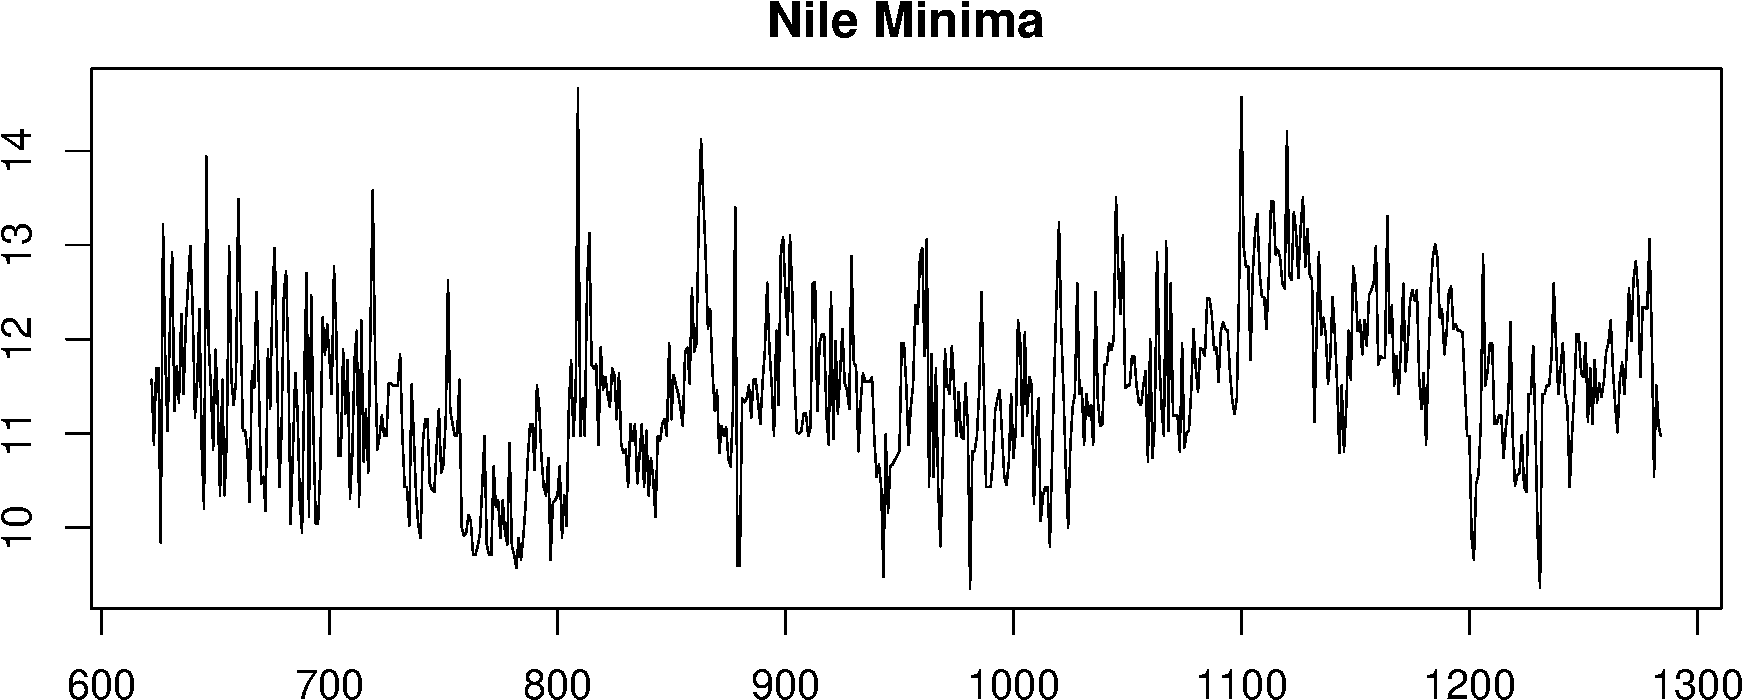
\includegraphics[width=\textwidth]{img/NileMin_ts.pdf}}
	\subcaptionbox{\label{fig:NileMin_acf}}{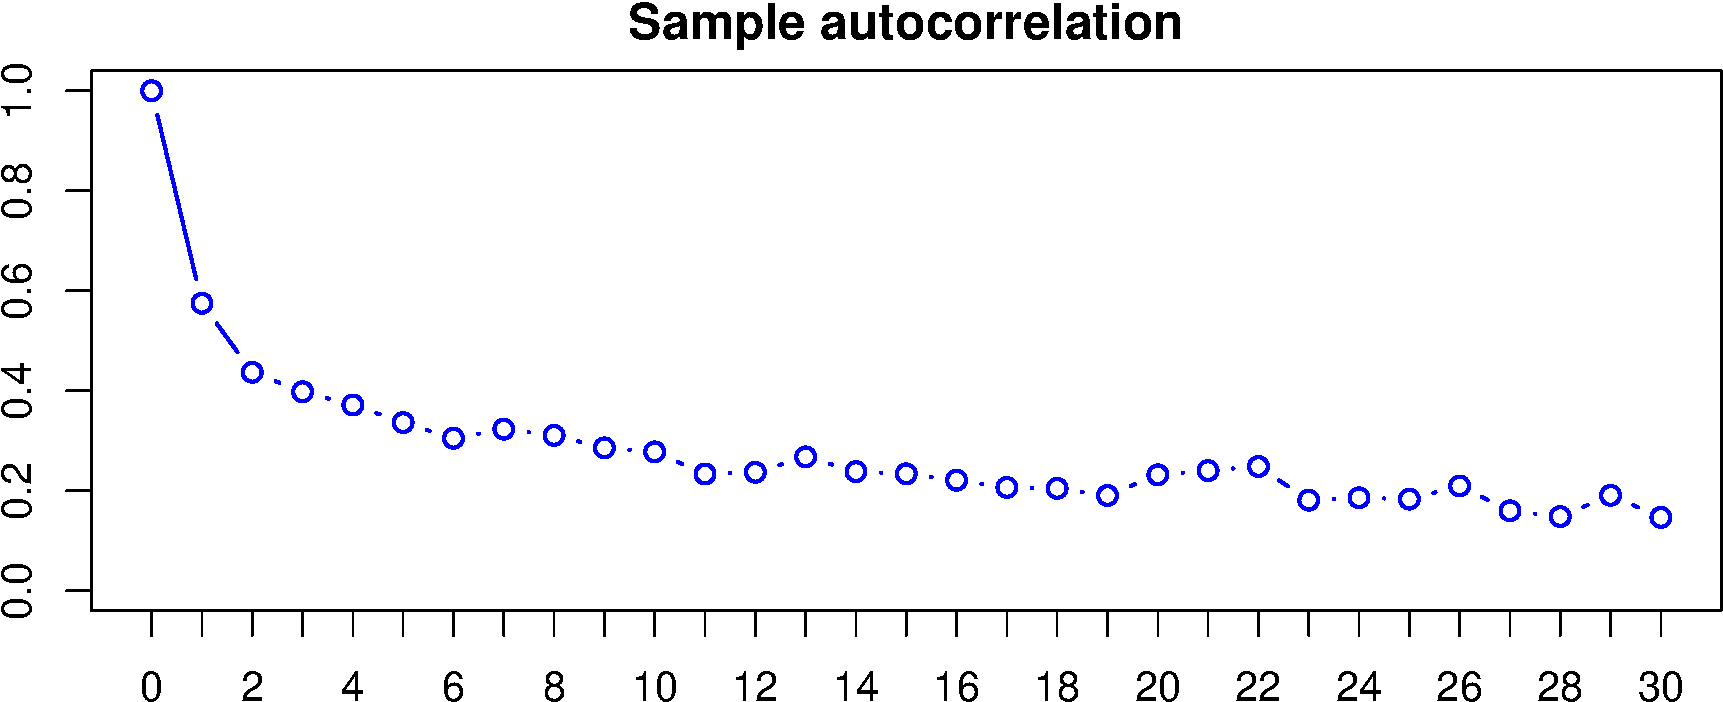
\includegraphics[width=\textwidth]{img/NileMin_acf.pdf}}
	\caption{Ежегодный минимальный уровень воды реки Нил}
\end{figure}

На рис.~\ref{fig:NileMin_ts} изображен ежегодный минимальный уровень воды реки Нил за период с 622 по 1284 год (663 наблюдения), данные были взяты из~\cite{Beran1994}. Нерегулярные циклы или тенденции в этом временном ряду, обусловленные длинной памятью, впервые были обнаружены и обсуждены Хёрстом, британским инженером, который работал гидрологом на реке Нил. Подтверждает присутсвие длинной памяти график медленно угасающей автокорреляционной функции на рис.~\ref{fig:NileMin_acf}.

\begin{table}[t]
	\centering
	\caption{Оценка параметров модели $\mathrm{ARFIMA}(0, d, 0)$ ряда Nile Minima}
	\label{tab:NileMin_est}
	\begin{tabular}{|c|c|c|}
		\hline
		Метод & $\hat{d}$ & $\hat{\sigma}^2$ \\
		\hline
		$\mathrm{MLE}(\bar x)$ & 0.39264 & 0.48939 \\
		H\&R & 0.39327 & 0.48934 \\
		Whittle & 0.40547 & 0.49026 \\
		\hline
	\end{tabular}
\end{table}

\begin{figure}[h]
	\centering
	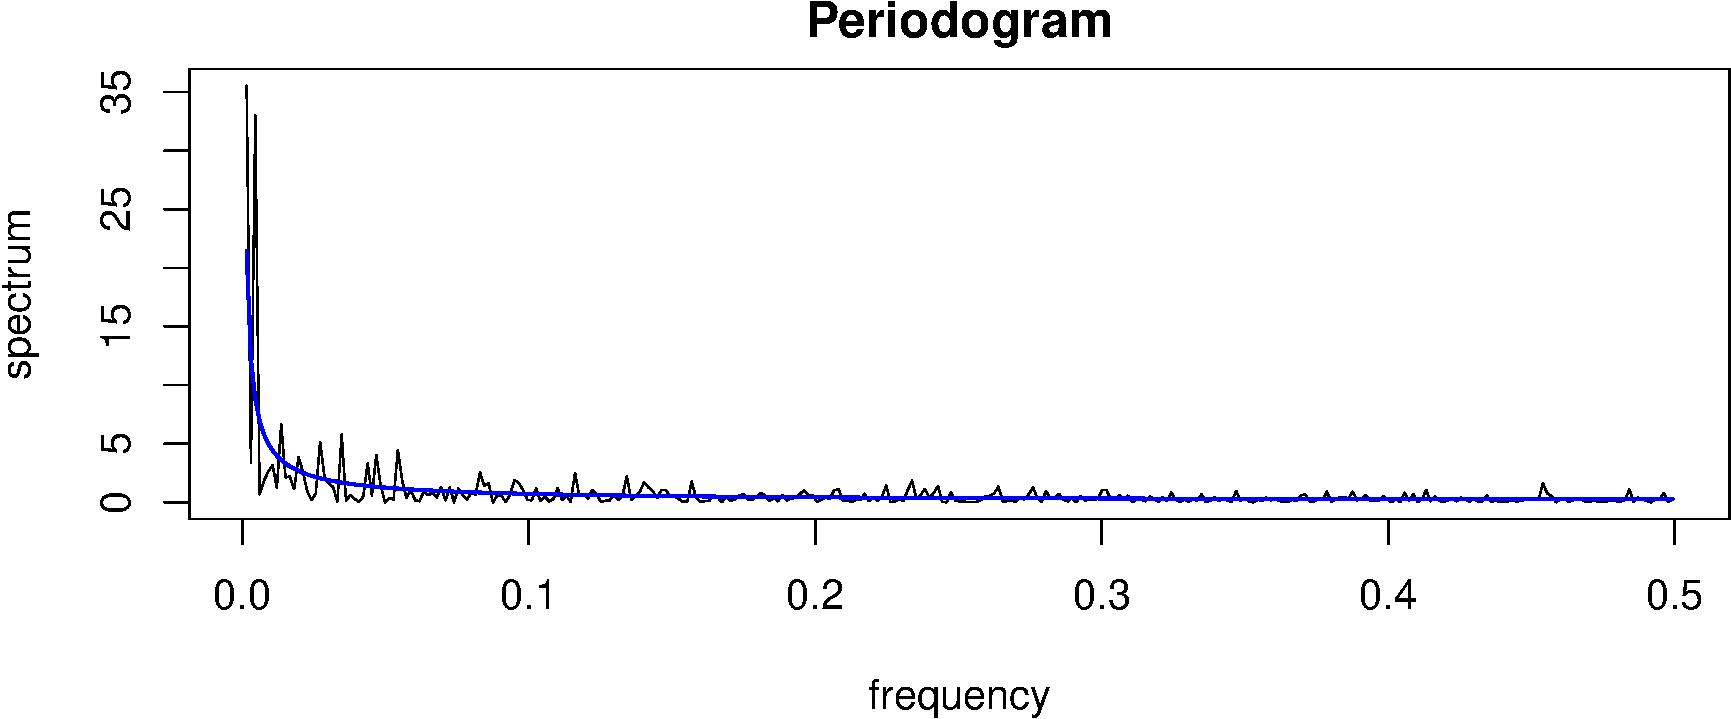
\includegraphics[width=\textwidth]{img/NileMin_per.pdf}
	\caption{Периодограмма ряда Nile Minima}
	\label{fig:NileMin_per}
\end{figure}

Оценим параметры модели $\mathrm{ARFIMA}(0, d, 0)$. В таблице~\ref{tab:NileMin_est} представлены оценки параметров $d$ и $\sigma^2$. Поскольку истинное среднее неизвестно и оценка $d$ по Whittle дает наименьшее смещение (см. рис.~\ref{fig:fi_est}), в качестве нулевой гипотезы MC-SSA выберем модель $\mathrm{ARFIMA}(0, d, 0)$ с $d=0.40547$ и $\sigma^2=0.48971$, на рис.~\ref{fig:NileMin_per} изображена периодограмма ряда вместе с оцененной спектральной плотностью.

\begin{figure}[h!]
	\centering
	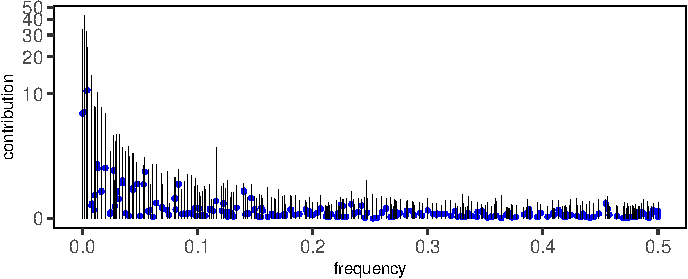
\includegraphics[width=\textwidth]{img/NileMin_mcssa.pdf}
	\caption{Результат работы MC-SSA для ряда Nile Minima}
	\label{fig:NileMin_mcssa}
\end{figure}

Применим MC-SSA с длиной окна $L=330\approx N / 2$. На рис.~\ref{fig:NileMin_mcssa} изображены 95\%-ные доверительные интервалы статистик $\widehat{p}_k$, $k=1,\ldots,L$ (см. алгоритм~\ref{alg:multiple_mc-ssa}). Ни одна из статистик не является значимой, это означает, что нет оснований полагать, что в этом временном ряде присутствует неслучайный сигнал.

\subsection{Ireland Wind}
На рис.~\ref{fig:IrelandWind_ts} изображены среднесуточные данные о скорости ветра (в узлах) за период с 1961 по 1978 год ($6574$ дней) на станции Roche's Point в Республике Ирландия~\cite{Haslett1989}. 

\begin{figure}[h]
	\centering
	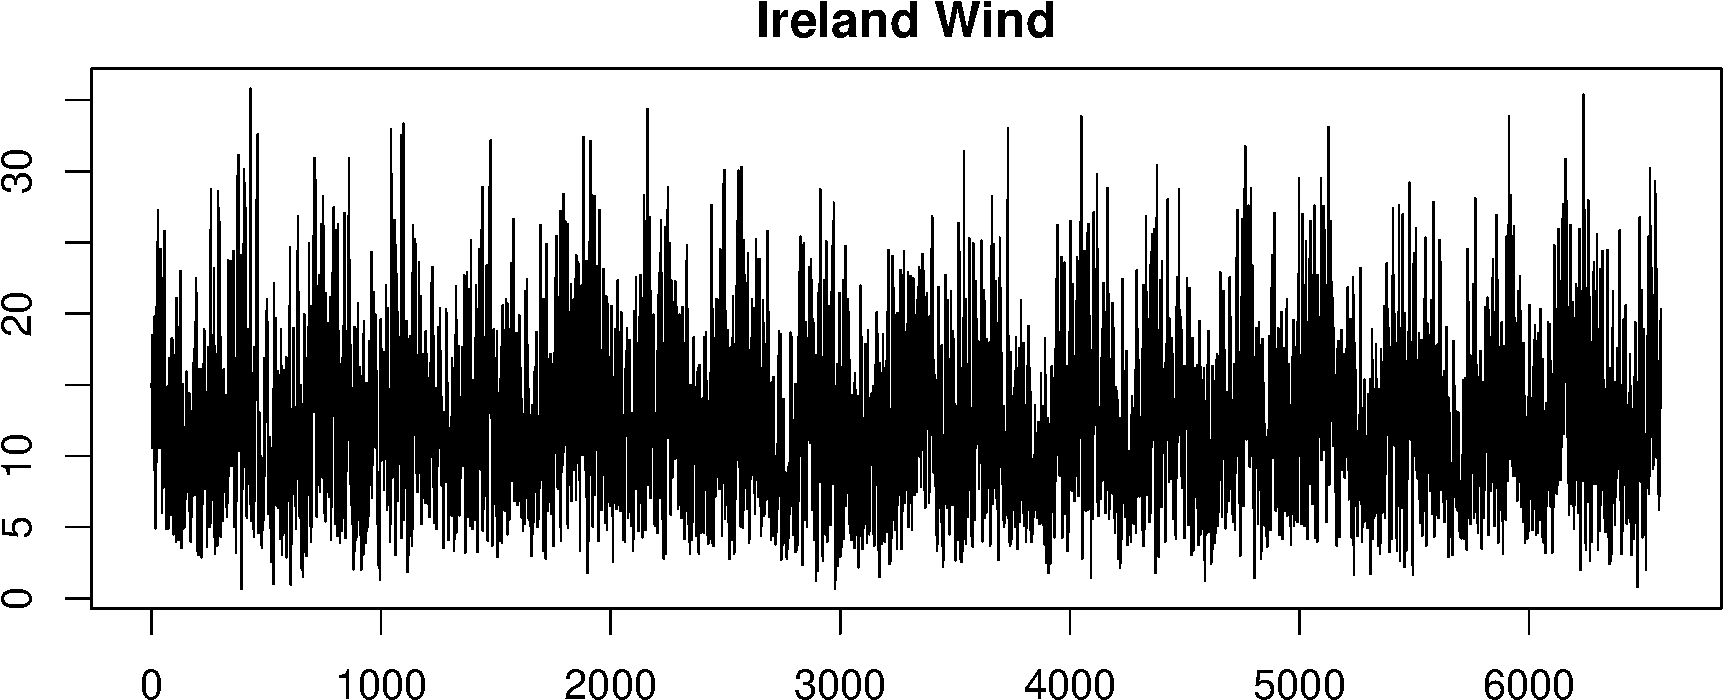
\includegraphics[width=\textwidth]{img/IrelandWind_ts.pdf}
	\caption{Среднесуточные данные о скорости ветра в Республике Ирландия}
	\label{fig:IrelandWind_ts}
\end{figure}

В таблице~\ref{tab:IrelandWind_est} представлены оценки параметров. Полученные оценки примерно одинаковые, но поскольу Whittle дает менее смещенную оценку (см. рис.~\ref{fig:fi_est} и таблицу~\ref{tab:arfi_est_n1000}), будем использовать именно ее.

\begin{table}[h]
	\centering
	\caption{Оценка параметров ряда Ireland Wind}
	\label{tab:IrelandWind_est}
	\begin{tabular}{|c|c|c|c|c|c|}
		\cline{2-6}
		\multicolumn{1}{c|}{} & \multicolumn{2}{c|}{$\mathrm{ARFIMA}(0, d, 0)$} & \multicolumn{3}{c|}{$\mathrm{ARFIMA}(1, d, 0)$} \\
		\hline
		Метод & $\hat d$ & $\hat\sigma^2$ & $\hat{d}$ & $\hat\phi$ & $\hat{\sigma}^2$ \\
		\hline
		$\mathrm{MLE}(\bar x)$ & 0.37117 & 24.39916 & 0.17306 & 0.28403 & 23.7581 \\
		H\&R & 0.36891 & 24.38116 & 0.17245 & 0.28309 & 23.73458 \\
		Whittle & 0.37287 & 24.40285 & 0.17598 & 0.28105 & 23.75983 \\
		\hline
	\end{tabular}
\end{table}

Поскольку ряд достаточно длинный, чтобы не делать поправку, рассмотрим в качестве векторов для проекции косинусы с равностоящими частотами с шагом $1/(2L)$. Также выберем длину окна не слишком большой, чтобы метод MC-SSA считался за адекватное время, скажем, $L=365$. На рис.~\ref{fig:IrelandWind_mcssa} представлен результат работы MC-SSA для обоих моделей, уровень значимости, как и в прошлом примере, равен $\alpha = 0.05$. Для модели $\mathrm{ARFIMA}(0, d, 0)$ значимых векторов два, их периоды равны $365 / 34\approx10.74$ и $365 / 60\approx6.08$ дней соответсвенно, что сложно как-то интерпретировать. Однако стоит заметить, что вклад значимых векторов не слишком превосходит верхнюю границу предсказательного интервала, поэтому, скорее всего, векторы значимы случайно (количество случайно значимых векторов в среднем равно $\alpha \cdot L=18.25$). В случае модели $\mathrm{ARFIMA}(1, d, 0)$ значим всего один вектор с периодом $365$ дней, что интерпретируется как наличие во временном ряде годовой периодичности.

% Получили следующее: если модель представляет собой чисто процесс с длинной памятью, много векторов оказывается значимыми, в то время как для модели, совмещающей в себе короткую и длинную память, значимых векторов уже нет. Но значимость векторов в первом случае может являться признаком неправильно выбранной модели. Также заметим, что критерий MC-SSA без поправки является радикальным, и значимые векторы могут на самом деле быть ложно обнаружеными. И поскольку применить поправку для такого длинного ряда не представляется возможным, интерпретировать полученный результат затруднительно. 

\begin{figure}[h!]
	\centering
	\subcaptionbox{$\mathrm{ARFIMA}(0, d, 0)$\label{fig:IrelandWind_mcssa_fi}}{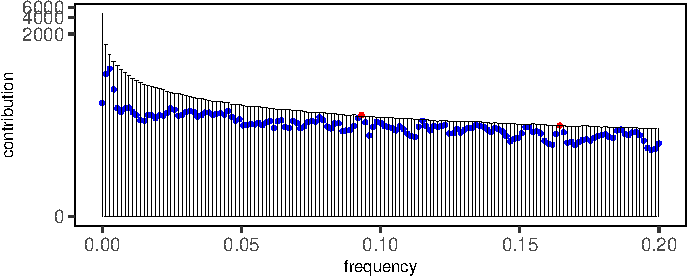
\includegraphics[width=\textwidth]{img/IrelandWind_mcssa_fi.pdf}}
	\subcaptionbox{$\mathrm{ARFIMA}(1, d, 0)$\label{fig:IrelandWind_mcssa_arfi}}{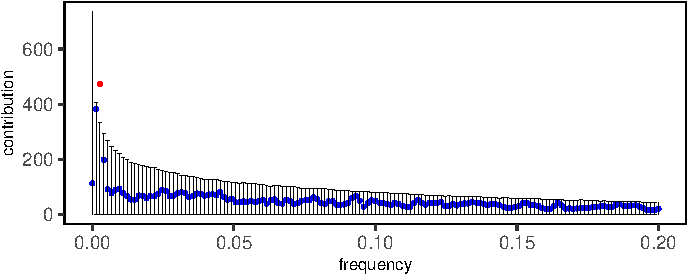
\includegraphics[width=\textwidth]{img/IrelandWind_mcssa_arfi.pdf}}
	\caption{Результат работы MC-SSA для ряда Ireland Wind}
	\label{fig:IrelandWind_mcssa}
\end{figure}

\conclusion
В ходе данной работы был реализован метод Monte Carlo SSA, когда в качестве модели шума рассматривается процесс с длинной памятью, а также его численное сравнение с Monte Carlo SSA с моделью красного шума, обладающей такой же дисперсией. Было получено, что если в качестве альтернативы рассмотреть сигнал с некоторой частотой, б\'{о}льшую мощность против этой альтернативы дает та модель шума, спектральная плотность которой в этой частоте наименьшая. 

Помимо этого, было проведено численное сравнение различных методов оценки параметров модели $\mathrm{ARFIMA}(p, d, q)$. Для этого были реализованы методы максимального правдоподобия и Whittle, а также были взяты функции из пакетов языка программирования \textsf{R}. Получено, что при известном среднем метод максимального правлоподобия является наилучшим методом, дающим наименьшую среднеквадратичную ошибку и смещение параметров. Если же среднее неизвестно, наиболее предпочтительным методом является Whittle.

\bibliographystyle{ugost2008}
\bibliography{report}

\appendix
\chapter{Графики}
\section{Сравнение \textsf{arfima\_mle} и \textsf{arfima}}\label{sect:mle_comparison}
На рис.~\ref{fig:mle_comparison_phi1},~\ref{fig:mle_comparison_phi5} и~\ref{fig:mle_comparison_phi9} представлены среднеквадратичное отклонение, смещение и дисперсия оценок параметров $\phi$ и $d$ модели $\mathrm{ARFIMA}(1, d, 0)$. По ним, видно, что при $\phi=0.1$ на рис.~\ref{fig:mle_comparison_phi1} оценки функцией \textsf{arfima} имеют скачок в $d=0.4$, что может говорить о некоторой вычислительной неустойчивости функции для больших $d$. Функция \textsf{arfima\_mle} не только не имеет подобной проблемы, но и дает более точные оценки, например, при $\phi=0.5$ на рис.~\ref{fig:mle_comparison_phi5}.

\begin{figure}[h]
	\centering
	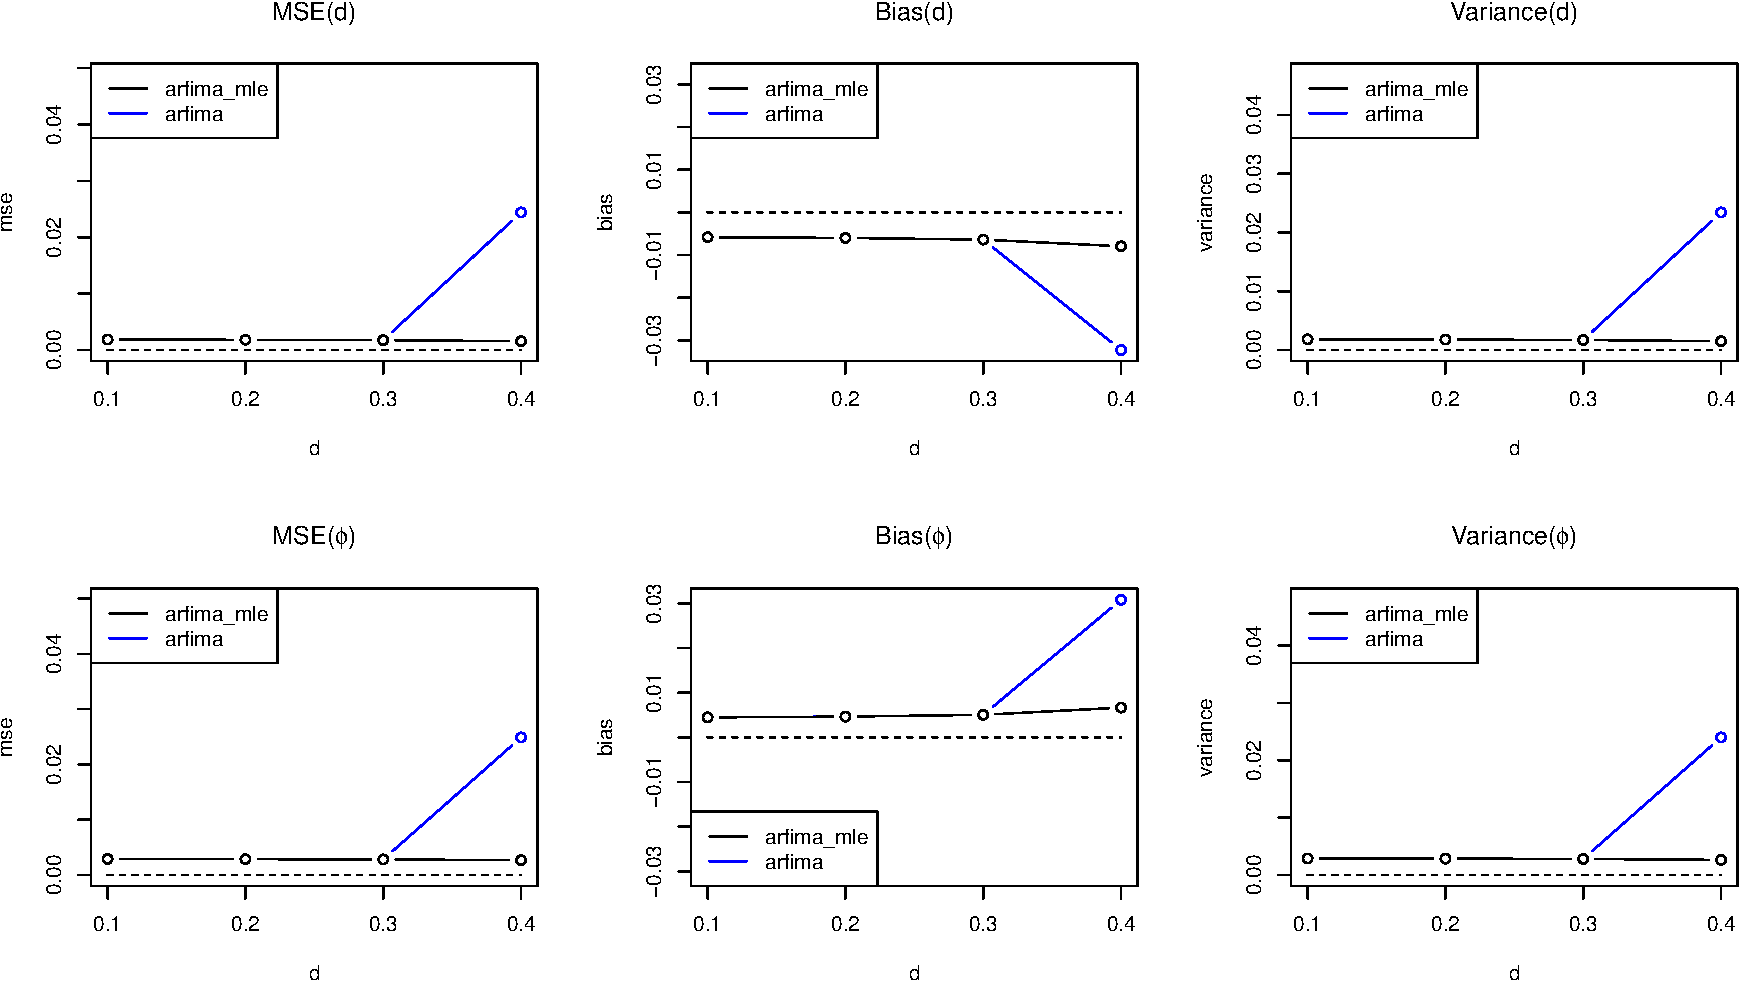
\includegraphics[width=\textwidth]{img/arfi_est_phi1.pdf}
	\caption{Сравнение \textsf{arfima\_mle} и \textsf{arfima} при $\phi=0.1$ ($n=1000$, $500$ повторений)}
	\label{fig:mle_comparison_phi1}
\end{figure}

\begin{figure}[h]
	\centering
	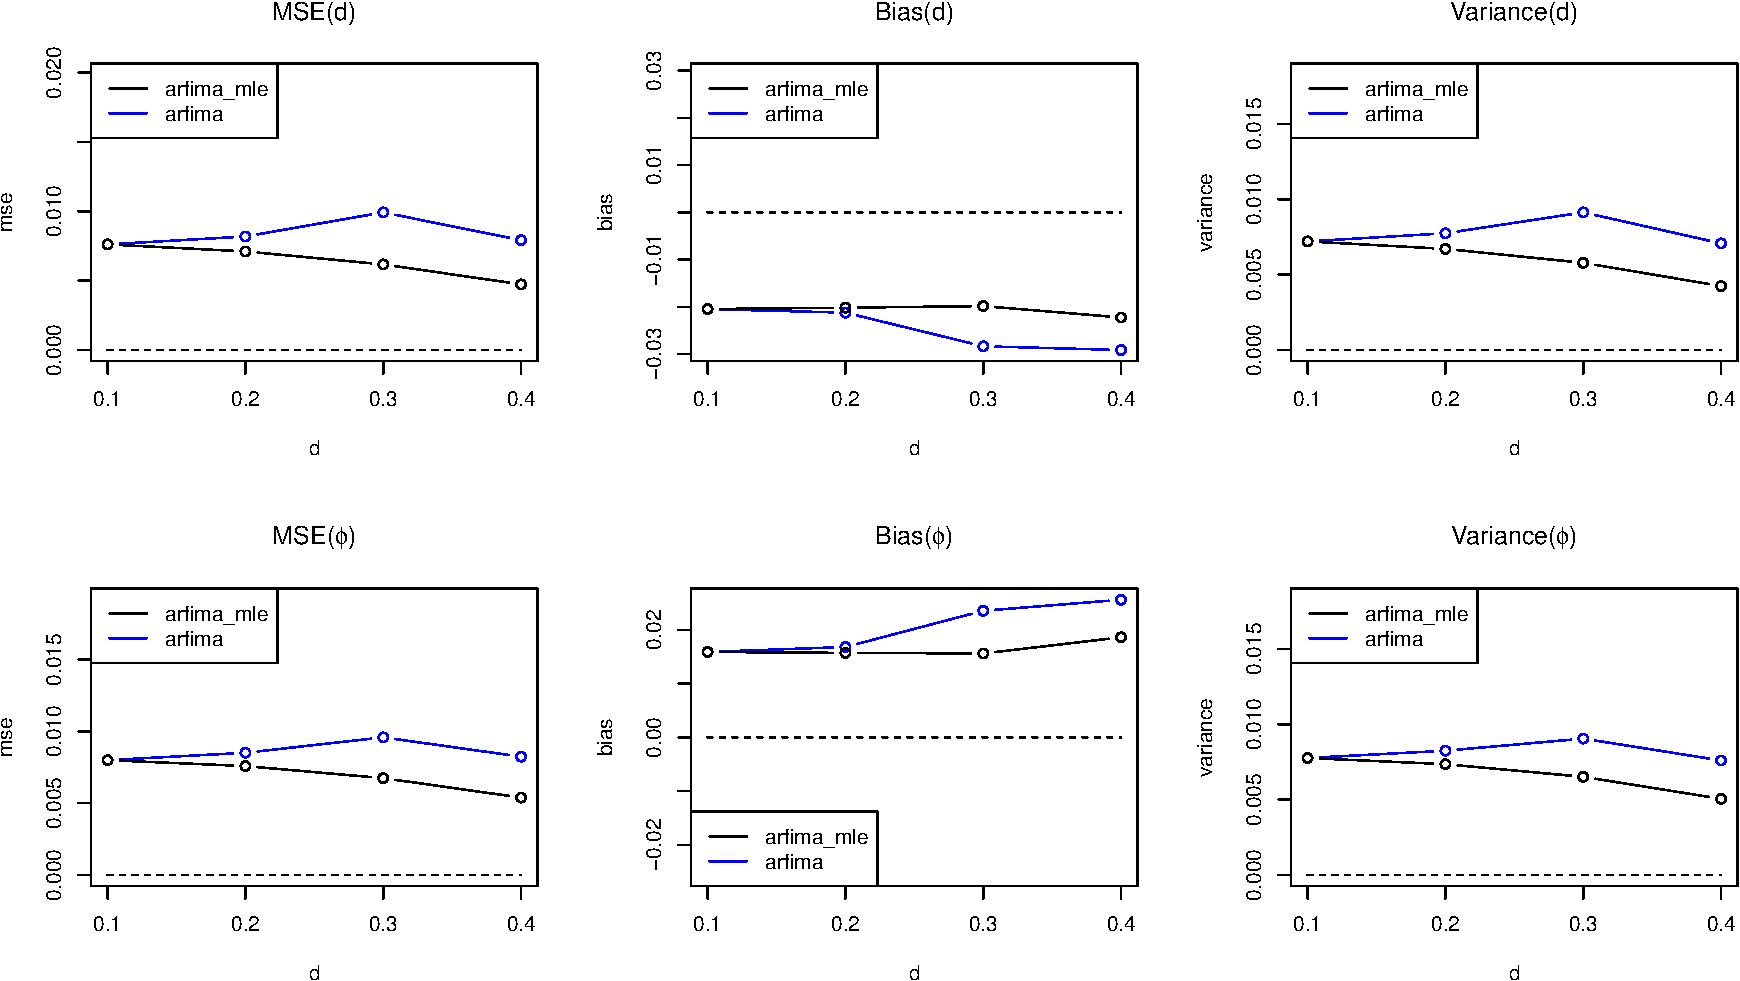
\includegraphics[width=\textwidth]{img/arfi_est_phi5.pdf}
	\caption{Сравнение \textsf{arfima\_mle} и \textsf{arfima} при $\phi=0.5$ ($n=1000$, $500$ повторений)}
	\label{fig:mle_comparison_phi5}
\end{figure}

\begin{figure}[h]
	\centering
	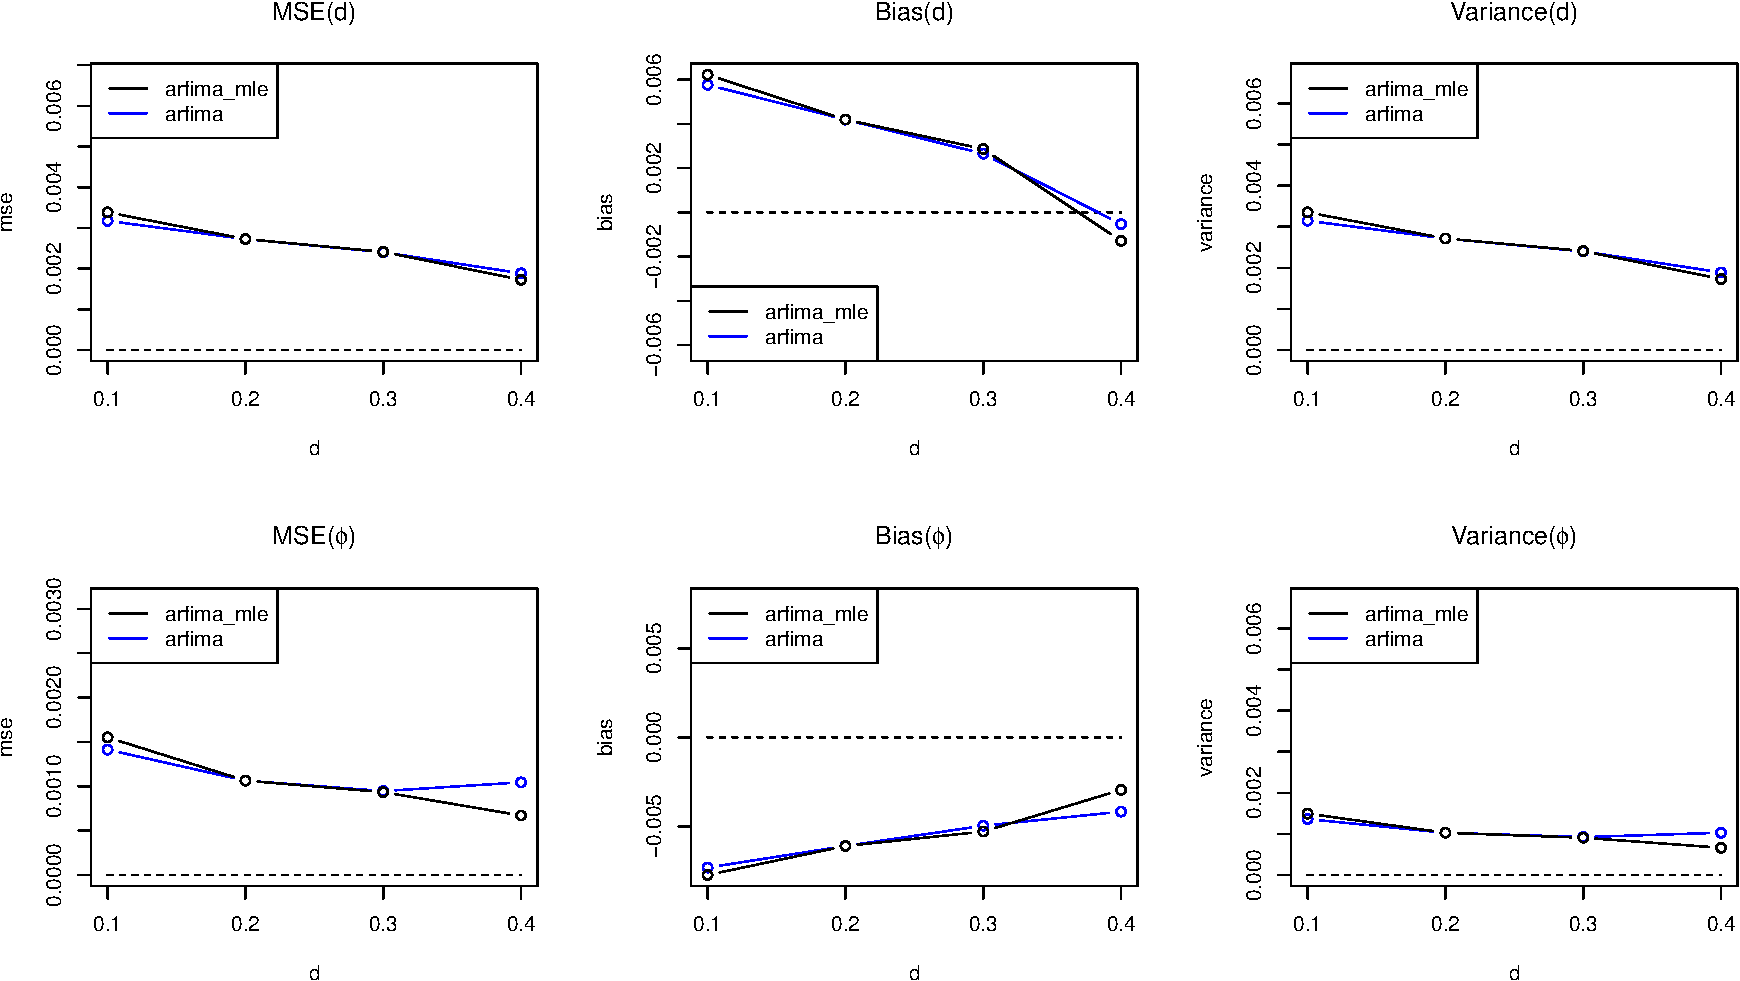
\includegraphics[width=\textwidth]{img/arfi_est_phi9.pdf}
	\caption{Сравнение \textsf{arfima\_mle} и \textsf{arfima} при $\phi=0.9$ ($n=1000$, $500$ повторений)}
	\label{fig:mle_comparison_phi9}
\end{figure}

\end{document}
